\documentclass[12pt,a4paper]{article}
\usepackage[utf8]{inputenc}
\usepackage[T1]{fontenc}
\usepackage[english]{babel}
\usepackage[english]{isodate}
\usepackage[paper=a4paper]{geometry}
\newgeometry{top=3.5cm,bottom=2.5cm,right=2.5cm,left=2.5cm}
\usepackage{graphicx}
\usepackage{comment}
\usepackage{fancyhdr}
\usepackage{framed}
\usepackage{lastpage}
\usepackage[hidelinks]{hyperref}
\usepackage{tabularx}
\usepackage[table]{xcolor}
\usepackage{enumitem}
\usepackage{mdwlist}
\usepackage{placeins}
\usepackage{amsmath}
\usepackage{xcolor}
\usepackage{listings}
\usepackage{amssymb}
\usepackage{amsthm}
\usepackage{xparse}
\usepackage{float}
\usepackage{chngcntr}

\counterwithin*{equation}{section}
\counterwithin*{equation}{subsection}


\begin{document}

\newcommand{\titolo}{Advanced Data Management}
\newcommand{\versione}{2.0}

\newcommand{\imageB}[2]{ 
        % 1 = image 
        % 2 = size
	\begin{figure}[h!]
    	\centering
    	\includegraphics[scale = #2]{img/#1} 
	\end{figure}
}

\newcommand{\image}[3]{
        % 1 = image 
        % 2 = size
        % 3 = caption
        \begin{figure}[h!]
    	\centering
    	\includegraphics[scale = #2]{img/#1} 
    	\caption{#3}
	\end{figure}
}

\newcommand{\imageLabel}[4]{ 
        % 1 = image 
        % 2 = size
        % 3 = caption
        % 4 = label
	\begin{figure}[h!]
    	\centering
    	\includegraphics[scale = #2]{img/#1} 
            \label{#4}
    	\caption{#3} 
	\end{figure}
}

\newcommand{\Z}{\mathbb{Z}}

\newcommand{\definition}[2]{
\vspace{3mm} \textbf{Definition (#1).} \textit{#2} \vspace{3mm}
}

\newcommand{\example}[1]{
\vspace{3mm} \textbf{Example.} \textit{#1} \vspace{3mm}
}

\newcommand{\theorem}[1]{
\vspace{3mm} \textbf{Theorem.} \textit{#1} \vspace{1mm}
}

\newcommand{\theoremNum}[2]{
\vspace{3mm} \textbf{Theorem #1.} \textit{#2} \vspace{1mm}
}

\newcommand{\theoremName}[2]{
\vspace{3mm} \textbf{Theorem (#1).} \textit{#2} \vspace{1mm}
}

\newcommand{\theoremBox}[1]{
\vspace{3mm} \begin{tcolorbox} \textbf{Theorem.} \textit{#1} \end{tcolorbox} \vspace{1mm}
}

\newcommand{\theoremNameBox}[2]{
\vspace{3mm} \begin{tcolorbox} \textbf{Theorem (#1).} \textit{#2} \end{tcolorbox} \vspace{1mm}
}

\newcommand{\theoremNumBox}[2]{
\vspace{3mm} \begin{tcolorbox} \textbf{Theorem #1.} \textit{#2} \end{tcolorbox} \vspace{1mm}
}

\newcommand{\lemma}[2]{
\vspace{3mm} \textbf{Lemma #1.} \textit{#2} \vspace{1mm}
}

\newcommand{\lemmaName}[2]{
\vspace{3mm} \textbf{Lemma (#1).} \textit{#2} \vspace{1mm}
}

\newcommand{\claim}[1]{
\vspace{3mm} \textbf{Claim.} \textit{#1} \vspace{1mm}
}

\pagenumbering{Alph}
\begin{titlepage}
	\begin{center}
		
\includegraphics[width=0.6\textwidth]{unive}
		
		\vspace*{1cm}
		\LARGE
		%\textit{Foundations of Machine Learning \\
	%		\center Year: 2022/2023}
		
		\vspace{0.5cm}
		\Huge
		\textbf{\titolo}\\
		
		\line(1,0){280}
		
		\vspace{0.5cm}
		\large
		\textit{Academic Year 2023/2024}
		
		\vfill
		
	\end{center}
	\begin{raggedleft}
		\Large
		%Team: \textbf{PeP4\_} \\
		\large
		Nicola Aggio 880008\\
	\end{raggedleft}
\end{titlepage}

%%%%%%%%%%%%%%%%%%%%%%%%%%%%%%%%%%%%%%%%%%%%%%%%%%%%%%%%%%%%%%%%%%%%%%%%%%%%%%%%
%% STILE HEADER - FOOTER - LISTE
%%%%%%%%%%%%%%%%%%%%%%%%%%%%%%%%%%%%%%%%%%%%%%%%%%%%%%%%%%%%%%%%%%%%%%%%%%%%%%%%

\renewcommand{\headheight}{14pt}

\pagestyle{fancy}
\lhead{}
\chead{}
\lhead{}
\rhead{\textbf{\titolo}}
\cfoot{}
\renewcommand{\headrulewidth}{0.4pt}
\renewcommand{\footrulewidth}{0.4pt}

%\renewcommand{\labelitemii}{$\bullet$}
%\renewcommand{\labelitemiii}{$\circ$}

\setlist{itemsep=0pt}

\setlength{\parindent}{0cm}

%%%%%%%%%%%%%%%%%%%%%%%%%%%%%%%%%%%%%%%%%%%%%%%%%%%%%%%%%%%%%%%%%%%%%%%%%%%%%%%%
%% INDICE
%%%%%%%%%%%%%%%%%%%%%%%%%%%%%%%%%%%%%%%%%%%%%%%%%%%%%%%%%%%%%%%%%%%%%%%%%%%%%%%%

\pagenumbering{gobble}
\renewcommand{\contentsname}{Index}
\tableofcontents
\newpage
\pagenumbering{arabic}

%%%%%%%%%%%%%%%%%%%%%%%%%%%%%%%%%%%%%%%%%%%%%%%%%%%%%%%%%%%%%%%%%%%%%%%%%%%%%%%%
%% FOOTER CON NUMERO PAGINA
%%%%%%%%%%%%%%%%%%%%%%%%%%%%%%%%%%%%%%%%%%%%%%%%%%%%%%%%%%%%%%%%%%%%%%%%%%%%%%%%

\rfoot{\thepage\ of \pageref{LastPage}}

\definecolor{mygreen}{rgb}{0,0.6,0}
\definecolor{mygray}{rgb}{0.5,0.5,0.5}
\definecolor{mymauve}{rgb}{0.58,0,0.82}

\lstset{ %
	backgroundcolor=\color{white},   % choose the background color; you must add \usepackage{color} or \usepackage{xcolor}; should come as last argument
	basicstyle=\footnotesize,        % the size of the fonts that are used for the code
	breakatwhitespace=false,         % sets if automatic breaks should only happen at whitespace
	breaklines=true,                 % sets automatic line breaking
	captionpos=b,                    % sets the caption-position to bottom
	commentstyle=\color{mygreen},    % comment style
	deletekeywords={...},            % if you want to delete keywords from the given language
	escapeinside={\%*}{*)},          % if you want to add LaTeX within your code
	extendedchars=true,              % lets you use non-ASCII characters; for 8-bits encodings only, does not work with UTF-8
	frame=single,	                   % adds a frame around the code
	keepspaces=true,                 % keeps spaces in text, useful for keeping indentation of code (possibly needs columns=flexible)
	keywordstyle=\color{blue},       % keyword style
	language=Octave,                 % the language of the code
	morekeywords={*,...},            % if you want to add more keywords to the set
	numbers=left,                    % where to put the line-numbers; possible values are (none, left, right)
	numbersep=5pt,                   % how far the line-numbers are from the code
	numberstyle=\tiny\color{mygray}, % the style that is used for the line-numbers
	rulecolor=\color{black},         % if not set, the frame-color may be changed on line-breaks within not-black text (e.g. comments (green here))
	showspaces=false,                % show spaces everywhere adding particular underscores; it overrides 'showstringspaces'
	showstringspaces=false,          % underline spaces within strings only
	showtabs=false,                  % show tabs within strings adding particular underscores
	stepnumber=2,                    % the step between two line-numbers. If it's 1, each line will be numbered
	stringstyle=\color{mymauve},     % string literal style
	tabsize=2,	                   % sets default tabsize to 2 spaces
	title=\lstname                   % show the filename of files included with \lstinputlisting; also try caption instead of title
}

%Theorem definitions
\theoremstyle{plain}
\newtheorem{thm}{Theorem}[section] % reset theorem numbering for each chapter
\theoremstyle{definition}
\newtheorem{defn}[thm]{Definition} % definition numbers are dependent on theorem numbers
\newtheorem{exmp}[thm]{Example} % same for example numbers

\newcommand{\chaptercontent}{
	\section{Basics}
	\begin{defn}Here is a new definition.\end{defn}
	\begin{thm}Here is a new theorem.\end{thm}
	\begin{thm}Here is a new theorem.\end{thm}
	\begin{exmp}Here is a good example.\end{exmp}
	\subsection{Some tips}
	\begin{defn}Here is a new definition.\end{defn}
	\section{Advanced stuff}
	\begin{defn}Here is a new definition.\end{defn}
	\subsection{Warnings}
	\begin{defn}Here is a new definition.\end{defn}
}

\NewDocumentCommand{\ceil}{s O{} m}{%
	\IfBooleanTF{#1} % starred
	{\left\lceil#3\right\rceil} % \ceil*[..]{..}
	{#2\lceil#3#2\rceil} % \ceil[..]{..}
}

\section{Multidimensional data organizations}

\subsection{Types of data and queries}

Let's consider multidimensional data representing points or regions in a k-dimensional space.

An example could be the following: consider a set of 8 records with two attributes A1 and A2 of type integer, which represent the latitude and longitude of cities, whose name will be used to denote the corresponding record, as shown in Picure \ref{multi_1}. Picture \ref{multi_2} provides a 2-dimensional representation of the points.

\begin{figure}[h!]
		\centering
		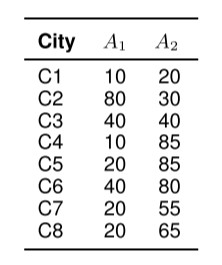
\includegraphics[scale = 1.5]{img/multi_1.jpg}
		\label{multi_1}
\end{figure}

\begin{figure}[h!]
		\centering
		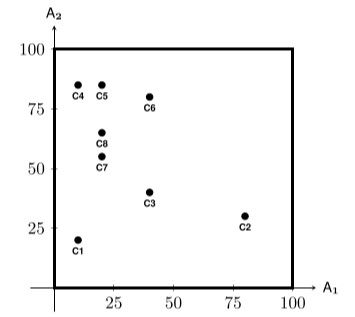
\includegraphics[scale = 1.5]{img/multi_2.jpg}
		\label{multi_2}
\end{figure}

The problems that will be considered are:

\begin{itemize}
    \item \textbf{primary organization}: how to divide stored data across pages;
    \item \textbf{secondary organization}: how to quickly find the region containing the points in a specified rectangular area. 
\end{itemize}

Both problems depend on the type of queries that are supported:

\begin{itemize}
    \item point/region search: check if a point/region is present;
    \item spatial range search: points/regions in a rectangle or ball;
    \item k-NN: find the k-closest points/regions with respect to a selected point/region.
\end{itemize}

\subsubsection{Multidimensional data organizations}
There exist different multidimensional data organizations.

\paragraph{Linear order based}
This organization let us to use traditional indexes in order to map positions, but it has a strong \textbf{precondition}: total order on the multidimensional data. Some examples of possible orders could be:

\begin{itemize}
    \item multi-attribute lexicographic order: in this case the points are store in a B+-tree. This order is useful for point search, but almost useless for range search and k-NN.

    \begin{figure}[h!]
		\centering
		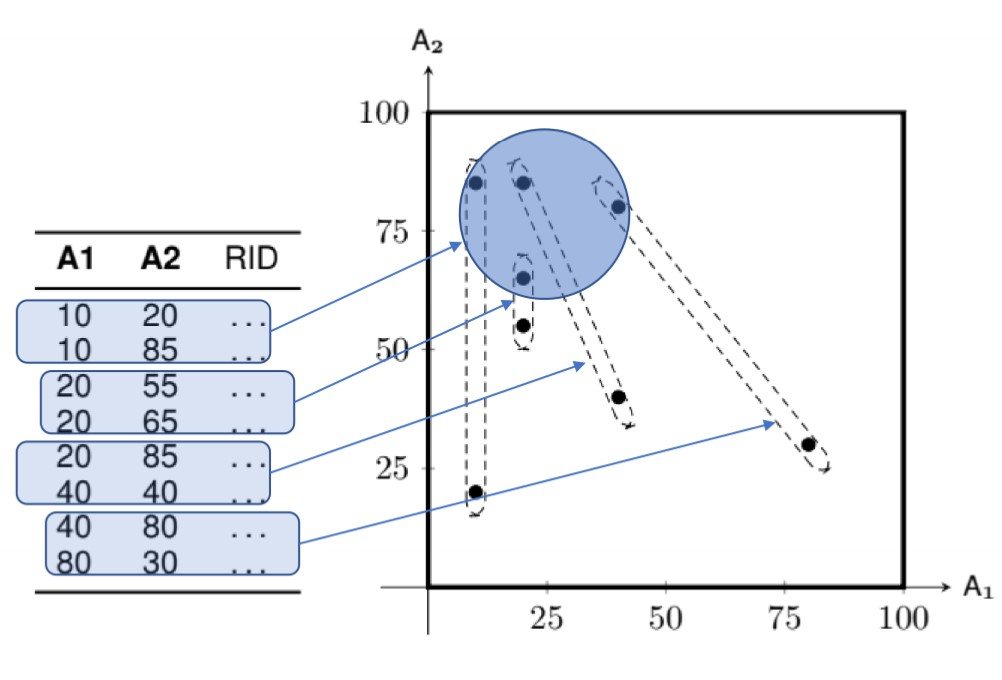
\includegraphics[scale = 0.8]{img/line1.jpg}
		\label{line1}
    \end{figure}

    \item diagonal order: in this case all the points are touched and it provides different type of granularity.

    \begin{figure}[H]
		\centering
		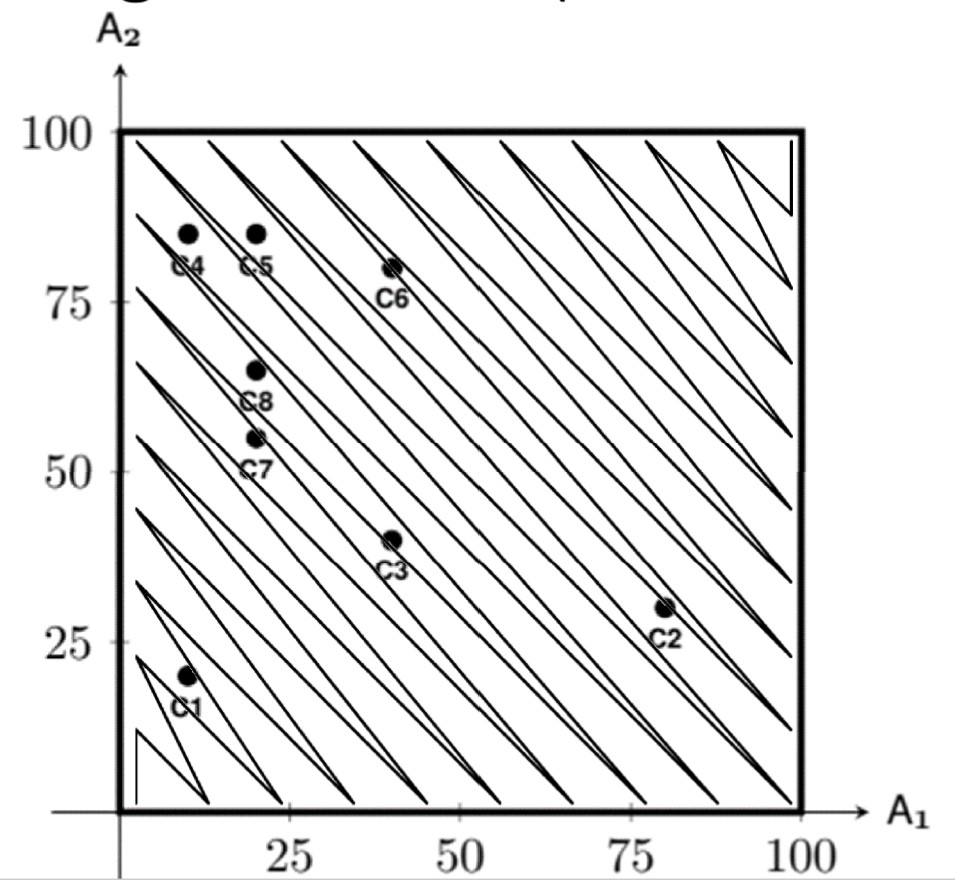
\includegraphics[scale = 0.7]{img/line2.jpg}
		\label{line2}
    \end{figure}

    \item Z-order

    \begin{figure}[h!]
		\centering
		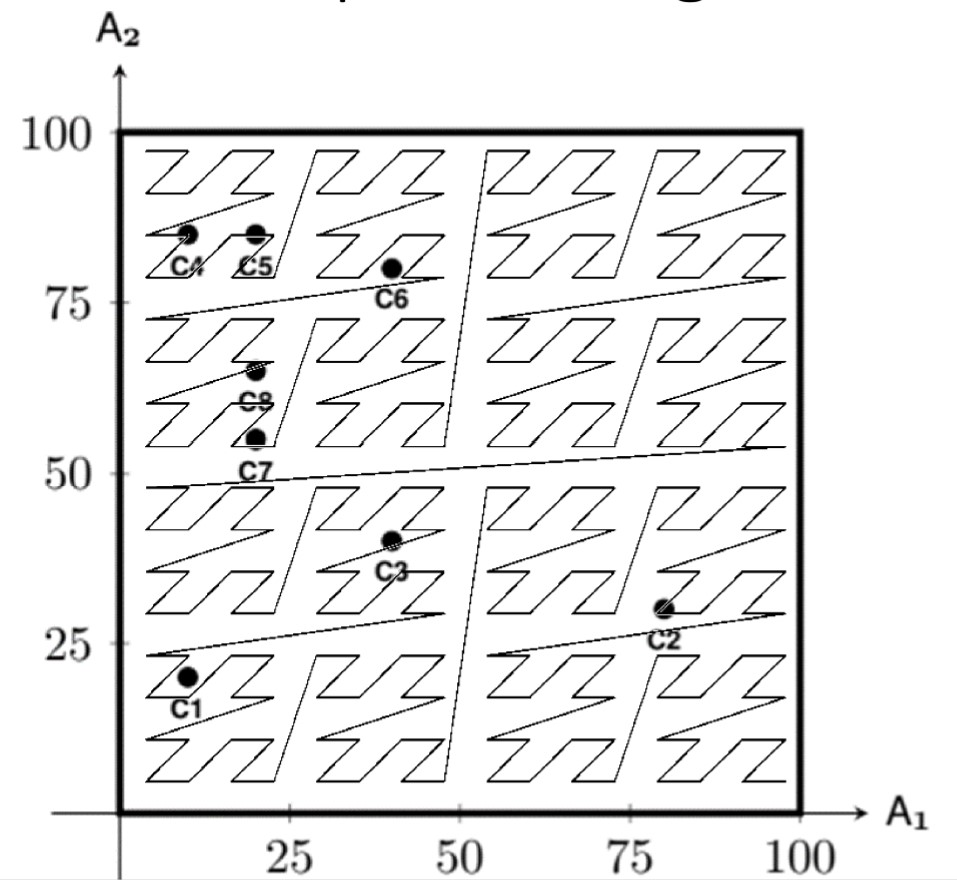
\includegraphics[scale = 0.7]{img/line3.jpg}
		\label{line3}
    \end{figure}

    \item Peano space filling curve

    \begin{figure}[h!]
		\centering
		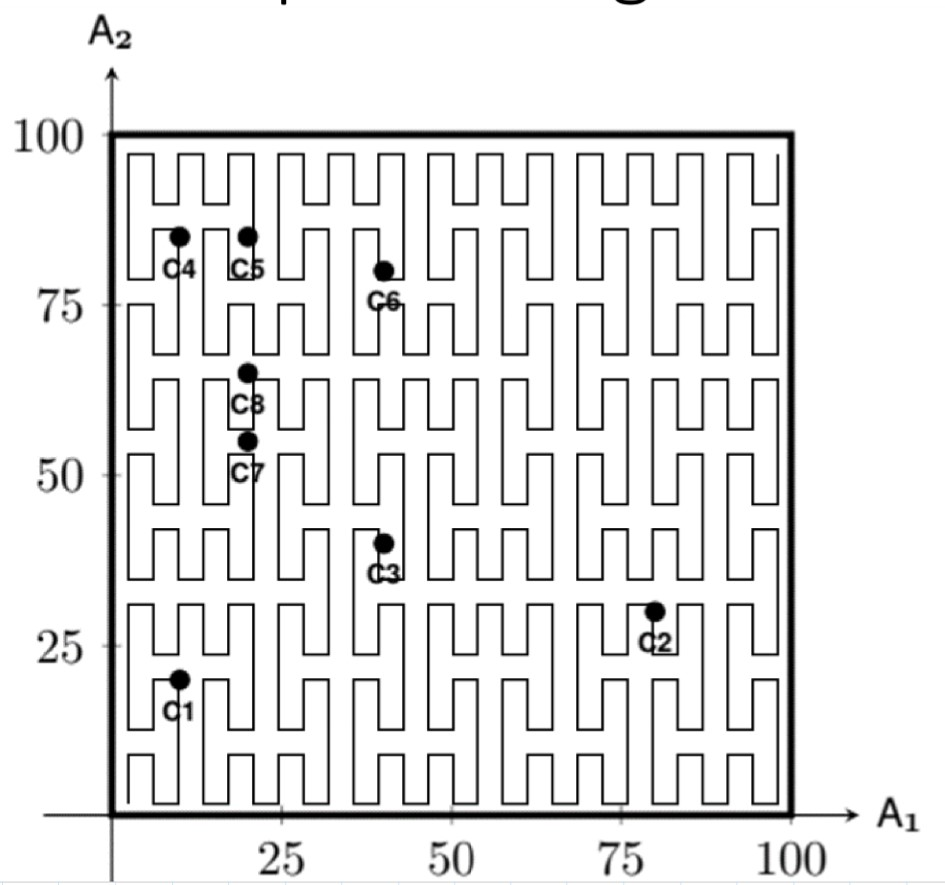
\includegraphics[scale = 0.7]{img/line5.jpg}
		\label{line5}
    \end{figure}

    \item Hilbert space filling curve

    \begin{figure}[H]
		\centering
		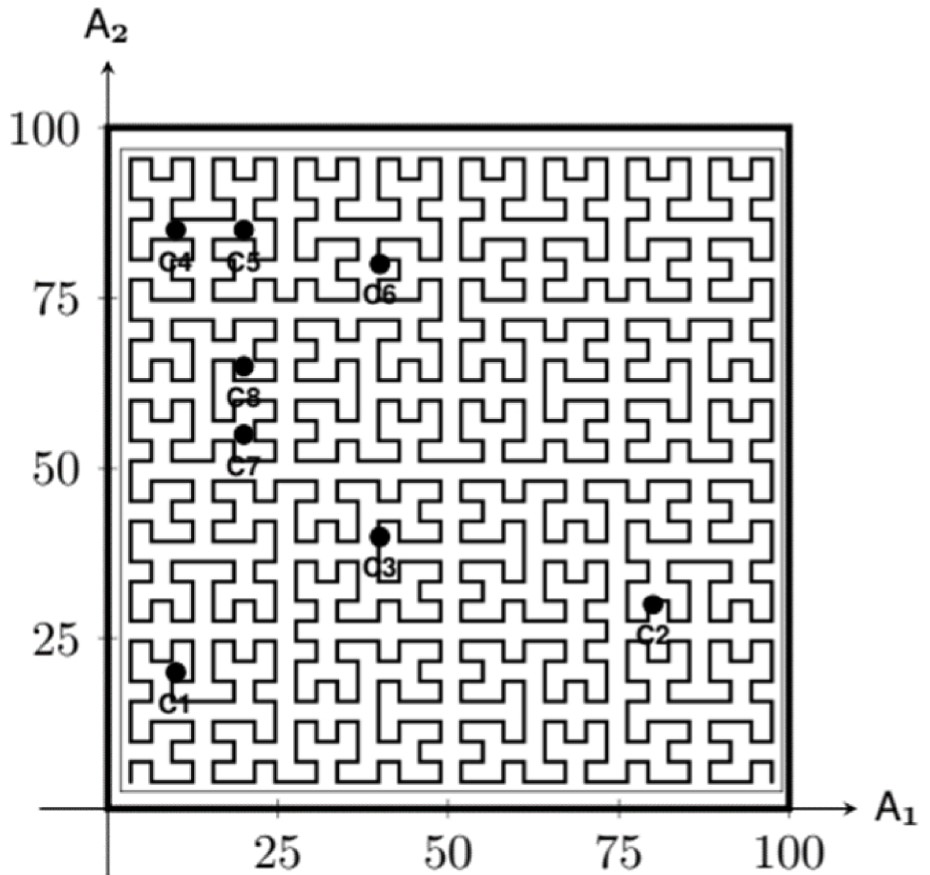
\includegraphics[scale = 0.7]{img/line4.jpg}
		\label{line4}
    \end{figure}
    
\end{itemize}

\subsubsection{Space partitioning}
In this case the focus is both on finding the partition of the space that results in (non-overlapping) regions that contain records that can be stored in a page and on how to quickly find the region containing the points for a specific query.

Let's focus on the different types of space partitioning:

\begin{itemize}
    \item classical partitioning: in this case the split is made according to a value of separation $d$ for a specific attribute. When there is a new overflow from a page during data loading, a new split is done, but changing the attribute.

    \begin{figure}[h!]
		\centering
		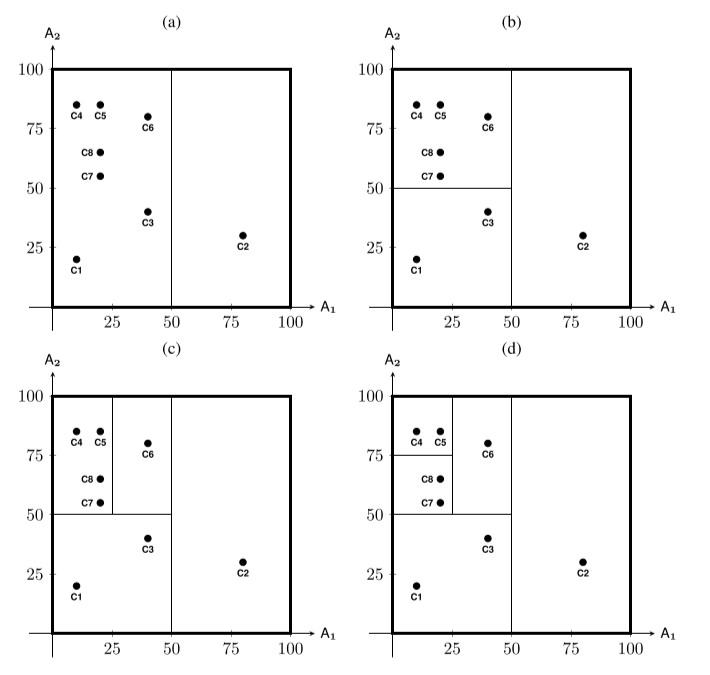
\includegraphics[scale = 1.2]{img/part1.jpg}
		\label{part1}
    \end{figure}

    \item point region quadtrees: this organization is used to organize bidimensional data, and it can be considered as the evolution of a binary tree into 2-dimension. Its limitation are:

    \begin{itemize}
        \item it is not balanced;
        \item it creates regions that are not needed;
        \item the higher the dimension, the higher the number of regions that are created.
    \end{itemize}

    \begin{figure}[h!]
		\centering
		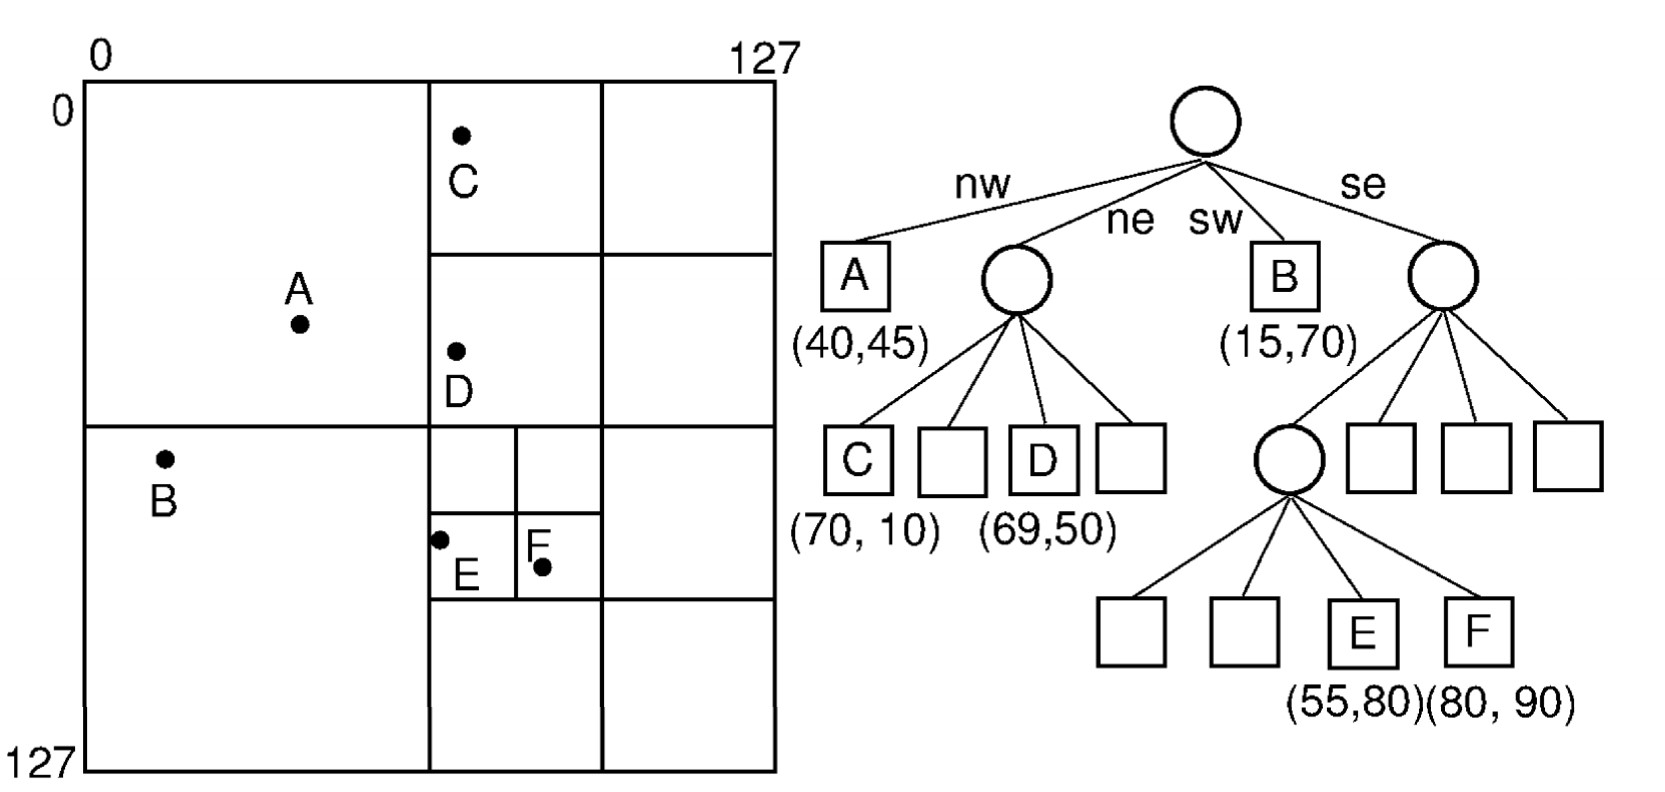
\includegraphics[scale = 0.5]{img/part2.jpg}
		\label{part2}
    \end{figure}

    
    \newpage
    \item octrees

    \begin{figure}[H]
		\centering
		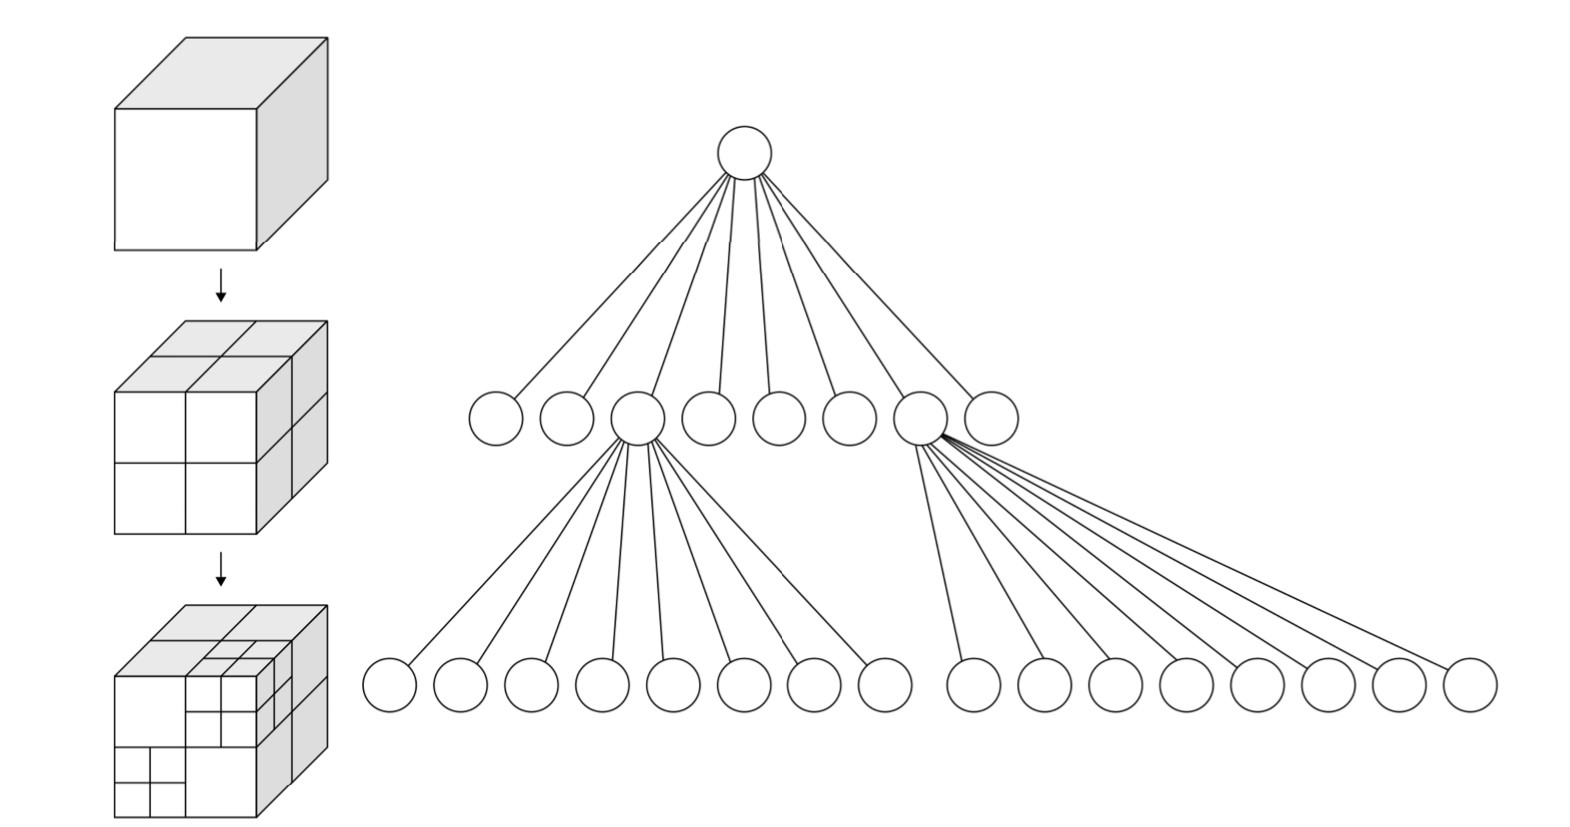
\includegraphics[scale = 0.5]{img/part3.jpg}
		\label{part3}
    \end{figure}

    \item KDB-trees: they inherit the idea of having a threshold to split the domain, but they use coordinates at time and they circle the order of the splitting strategy. In order to find the correct position, starting from the root is easier than starting from the leaves, because in this case an additional tree must be kept in order to manage the partition volume.

    \begin{figure}[h!]
		\centering
		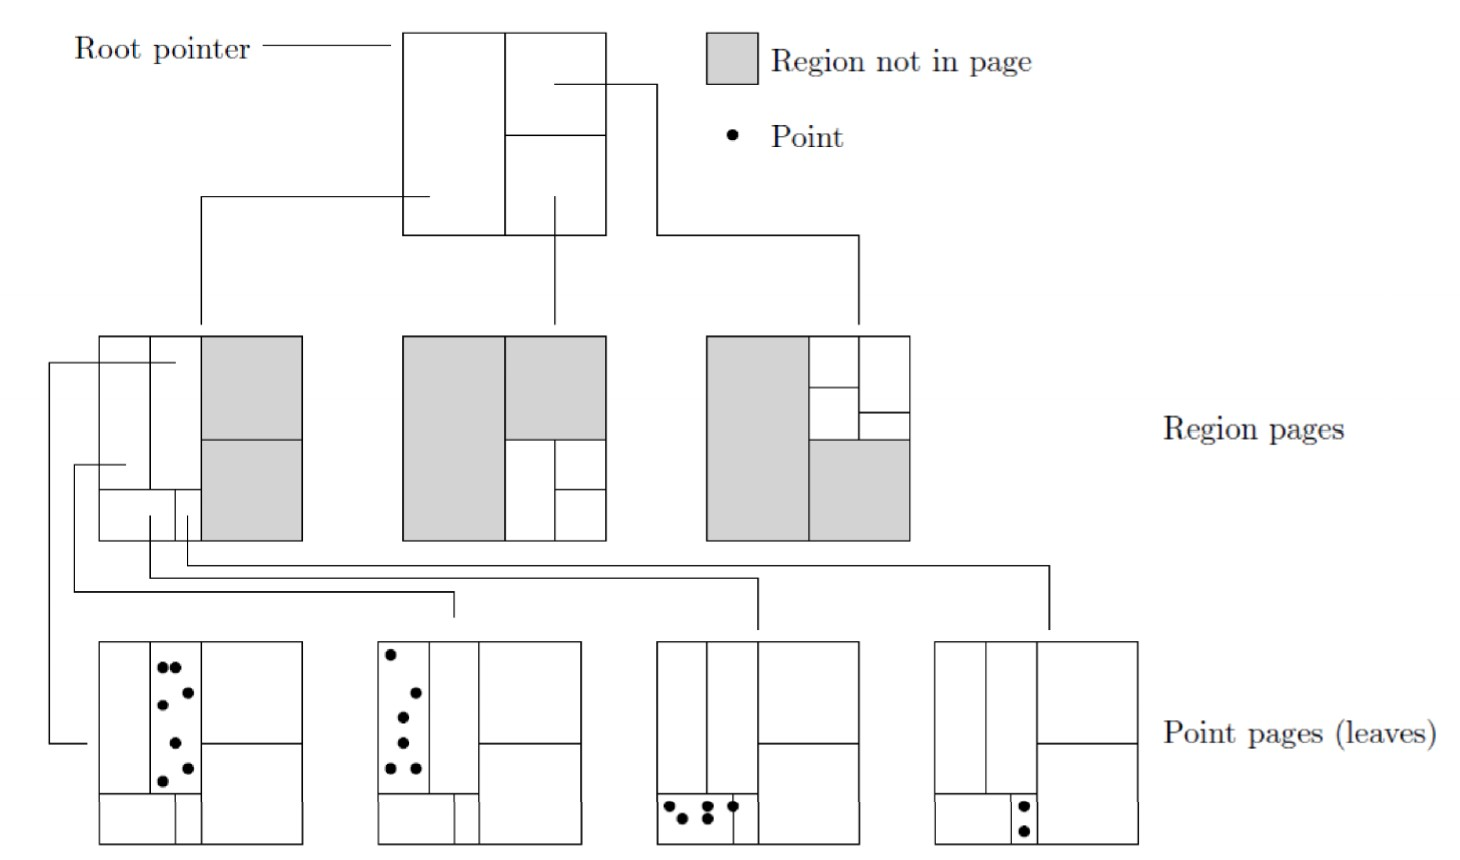
\includegraphics[scale = 0.7]{img/part4.jpg}
		\label{part4}
    \end{figure}
    
\end{itemize}

\subsubsection{G-trees}
\textbf{G-trees} combine the ideas of data partitioning and of B+-trees as follows: data space is divided into non-overlapping regions of variable size identified by an appropriate code, then a total ordering is defined for partition codes, and they're stored in a B+-tree. If we consider a 2-dimensional case, assuming that data pages may contain 2 points, then a \textbf{partition code} is a binary string constructed as follows:

\begin{itemize}
    \item the initial region is identified by the empty string;
    \item the first split is made along the X-axis, and the two partitions it produces are "0" and "1". Points $0 < x \leq 50$ are in partition "0", while points $50 < x \leq 100$ belong to partition "1";
    \item when a partition of the previous step is split along Y-axis, then the new partition codes become "00" and "01" and so on...
\end{itemize}

An example of G-tree is showed in Picture \ref{part5}.

\begin{figure}[H]
		\centering
		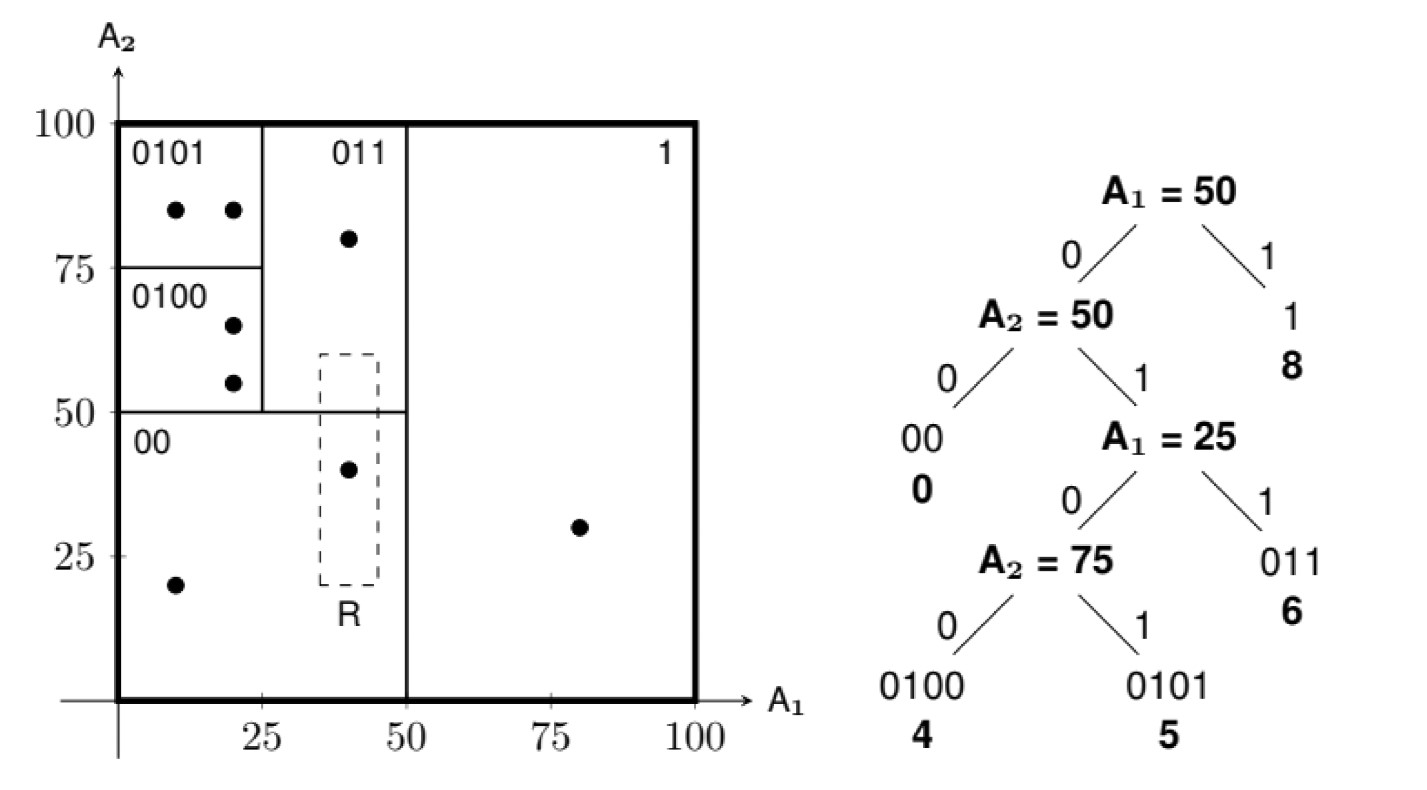
\includegraphics[scale = 0.7]{img/part5.jpg}
        \caption{Example of G-tree}
		\label{part5}
\end{figure}

The Picture \ref{part6} represents the partition codes and the B+-tree which is used to store them.

\begin{figure}[H]
		\centering
		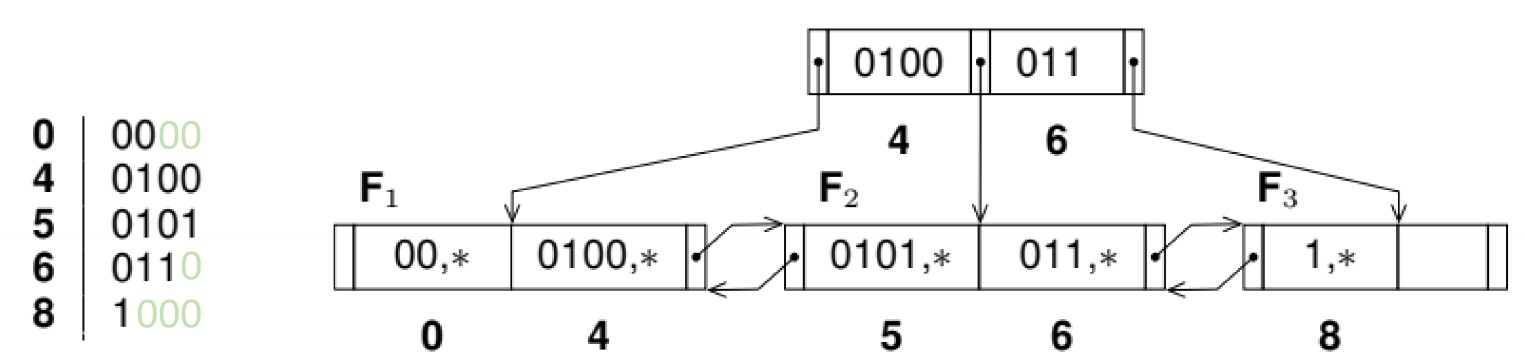
\includegraphics[scale = 0.7]{img/part6.jpg}
        \caption{Example of G-tree}
		\label{part6}
\end{figure}

\paragraph{Operations}

Now we focus on some possible operations which can be performed using these G-trees:

\begin{itemize}
    \item \textbf{point search}: let $M$ be the maximum length of the partition number of the G-tree, then the search for a point $P$ with coordinates $(x,y)$ proceeds as follows:

    \begin{enumerate}
        \item the partition tree is searched for the code $S_p$ of the partition that contains $P$, if it is present
        \item the G–tree is searched for the partition code $S_p$ to check if $P$ is in the associated page.
    \end{enumerate}
    
    \item \textbf{spatial range search}: a spatial range search looks for the points $P_i$ with coordinates $(x_i, y_i)$ such that $x_1 \leq x_i \leq x_2$ and $y_1 \leq y_i \leq y_2$, i.e. they are in the query region $R = \{ (x_1, y_1), (x_2, y_2) \}$. The query result is found as follows:

    \begin{enumerate}
        \item the G–tree is searched for the leaf node $F_h$ of the partition containing the lower left vertex $(x_1, y_1)$ of $R$
        \item the G–tree is searched for the leaf node $F_k$ of the partition containing the upper right vertex $(x_2, y_2)$ of $R$
        \item for each leaf from $F_h$ to $F_k$ the elements S are searched such that $R_S = RegionOf(S)$ overlaps with the query region $R$, where $RegionsOf(S)$ is a function that maps the code $S$ of a partition R in the coordinates of the lower left and upper right vertices of the partition
    \end{enumerate}

    \item \textbf{point insertion}: 

    \begin{enumerate}
        \item the G–tree is searched for the leaf node $F$ of the partition $R_p$ that should contain it. Let $S_p$ be the code of $R_p$
        \item if $R_p$ is not full, insert $P$, otherwise $R_p$ is split in $R_p_1$ and $S_p_1$, with codes $S_p_1 = S_p$“0” and $S_p_2 = S_p$“1”. If the new strings have a length greater than $M$, $M$ takes the value $M+1$
        \item the points in $R_p$ and $P$ are distributed in $RP1$ and $R_P_2$. 
        \item the element ($S_p$, $p_R_p$) in the leaf $F$ is replaced by ($S_p_1$, $p_R_p_1$) and ($S_p_2$, $p_R_p_2$)
    \end{enumerate}

    \item \textbf{point deletion}:
    \begin{enumerate}
        \item let $F$ be the leaf node with the partition $R_p$ containing $P$, $S_p$ the partition code of $R_p$, and $S$' the partition code of $R$' obtained from $R_p$ with a split and therefore different from $S_p$ for the last bit only
        \item $P$ is deleted from $R_p$ and then two cases are considered:
        \begin{itemize}
            \item $R$' has been split:
            \begin{itemize}
                \item If the partition $R_p$ becomes empty, then $S_p$ is deleted
                \item Otherwise the operation terminates
            \end{itemize}
            \item $R$' has not been split:
            \begin{itemize}
                \item If the two partition cannot be merged, the operation terminates
                \item Otherwise the two partition are merged
            \end{itemize}
        \end{itemize} 
    \end{enumerate}
\end{itemize}

\subsubsection{R*-trees}
\begin{itemize}
    \item an R*-tree is a dynamic tree structure perfectly balanced as a B+-tree, used for retrieval of multidimensional data according to ita spatial position;
    \item terminal nodes of a R*-tree contain elements of the form $(R_i, O_i)$, where:
    \begin{itemize}
        \item $R_i$ is the rectangular data;
        \item $O_i$ is its reference to the data nodes; for simplicity we denote $O_i$ as *.
    \end{itemize}  
    \item non terminal nodes contain elements of type $(R_i, p_i)$, where 
    \begin{itemize}
        \item $p_i$ is a reference to the root of a subtree;
        \item $R_i$ is the minimum bounding rectangle countaining all rectangles associated with the child nodes.
    \end{itemize}
\end{itemize}

\begin{figure}[H]
		\centering
		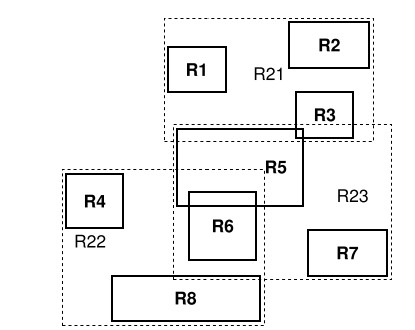
\includegraphics[scale = 1.3]{img/part7.jpg}
		\label{part6}
\end{figure}

\begin{figure}[H]
		\centering
		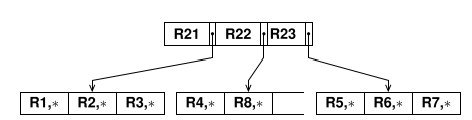
\includegraphics[scale = 1.5]{img/part8.jpg}
		\label{part6}
\end{figure}

The \textbf{properties} of R*-tree are:
\begin{itemize}
    \item each node has a number of elements between $m = $ the minimum number of elements in a node, and $M = $ the maximum;
    \item all leaf nodes are at the same level;
\end{itemize}

\textbf{Differences} with B+-trees:
\begin{itemize}
    \item there is no sort order in R*-trees, unlike B+-trees;
    \item there may be overlap between regions associated with different elements of the same level, unlike B+-trees.
\end{itemize}

\paragraph{Operations}

\begin{itemize}
    \item \textbf{search overlapping data regions}: suppose we want to search all the overlapping regions to the region $R$:
    \begin{itemize}
        \item the root is visited in order to look for elements $(R_i, p_i)$, with $R_i$ that overlaps with $R$;
        \item for each element $(R_i, p_i)$ found, the search proceeds in the subtree rooted in $p_i$: when a leaf node is reached, the data regions $R_i$ in the search results are those with $R_i$ that overlaps with $R$.
    \end{itemize}
    
    \begin{figure}[H]
		\centering
		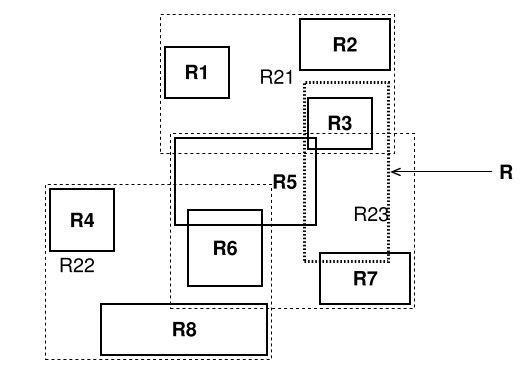
\includegraphics[scale = 1.5]{img/part9.jpg}
		\label{part6}
    \end{figure}
    
    In the example, $R_3, R_5$ and $R_7$ overlaps with $R$.

    \item \textbf{insertion}: let $S$ be a new data region to insert. The operation is similar to inserting a key in a B+-tree, since $S$ is stored in a leaf node, and if there is an overflow, the node will be split into two nodes. In the worst case the division can propagate to the parent node up to the root. However, there is a significant difference with the insertion in B+-trees: in R*-trees, since the regions may overlap, the new data region $S$ may overlaps with more of them, so it could be inserted in more leaf nodes. In this sense, the choice of the region in an internal node can be made according to the degree of overlap with $S$. After having selected the node $N$ where to insert $S$, if an overflow does not occur, the region is recalculated and its value propagates in the parent node, otherwise:

    \begin{enumerate}
        \item if it is the first overflow, then a fraction $p$ of the $M+1$ entries are removed from the node and reinserted in the tree, in a sort of dynamic reorganization of the tree
        \item otherwise, the $M+1$ elements are divided between two nodes, and two new elements are inserted in the parent node, and the process goes on to propagate the effects.
    \end{enumerate}

    \underline{Example}: assume to insert region $S$ (a): the process starts with the root node of the R*-tree in (c). Let the region $R21$ be selected for the insertion. Following the associated pointer, the leaf node to the left is considered, and since this node does not have enough space to contain $S$ an overflow occurs. Being the first, we proceed with the reinsertion of R1. The region $R21$ is updated (not shown in the figure) and the reinsertion takes place in the same leaf node, causing another overflow and then a subdivision. Suppose that we get ${R1, S}$ and ${R2, R3}$. Let $R24$ and $R25$ be the regions containing $(R1, S)$ and $(R2, R3)$ (b). Consequently, two new elements have to be inserted into the root node to replace $R21$ (c). Since in the root node there is not enough space to contain four elements, there is an overflow. In the root the reinsertion it is not applied, but a subdivision is made. The result is that the old root node is replaced by two new nodes, one containing $(R24, R25)$ and the other $(R22, R23)$. Let $R26$ be the region containing $(R24, R25)$ and $R27$ be the region containing $(R22, R23)$. A new root is added with elements $R26$ and $R27$ (d).

    \begin{figure}[h!]
		\centering
		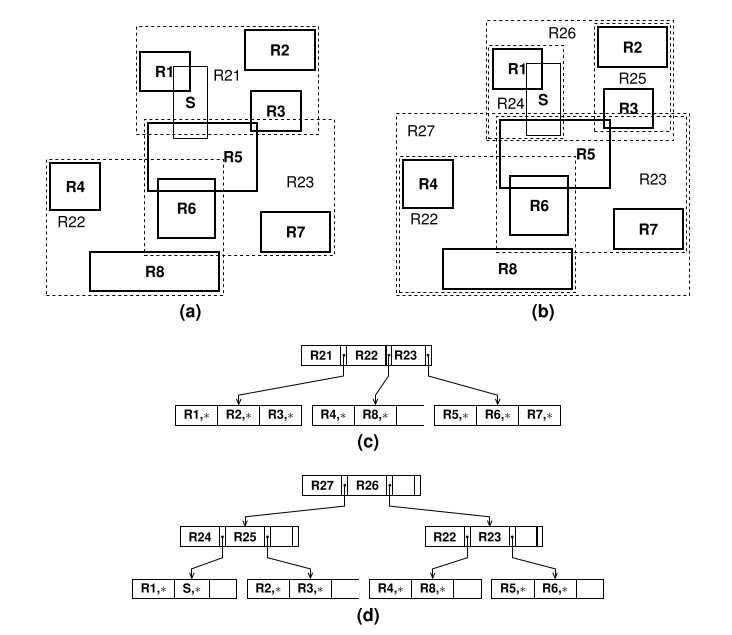
\includegraphics[scale = 1.6]{img/part10.jpg}
		\label{part6}
    \end{figure}
\end{itemize}
\section{Access methods management}

\begin{figure}[h!]
		\centering
		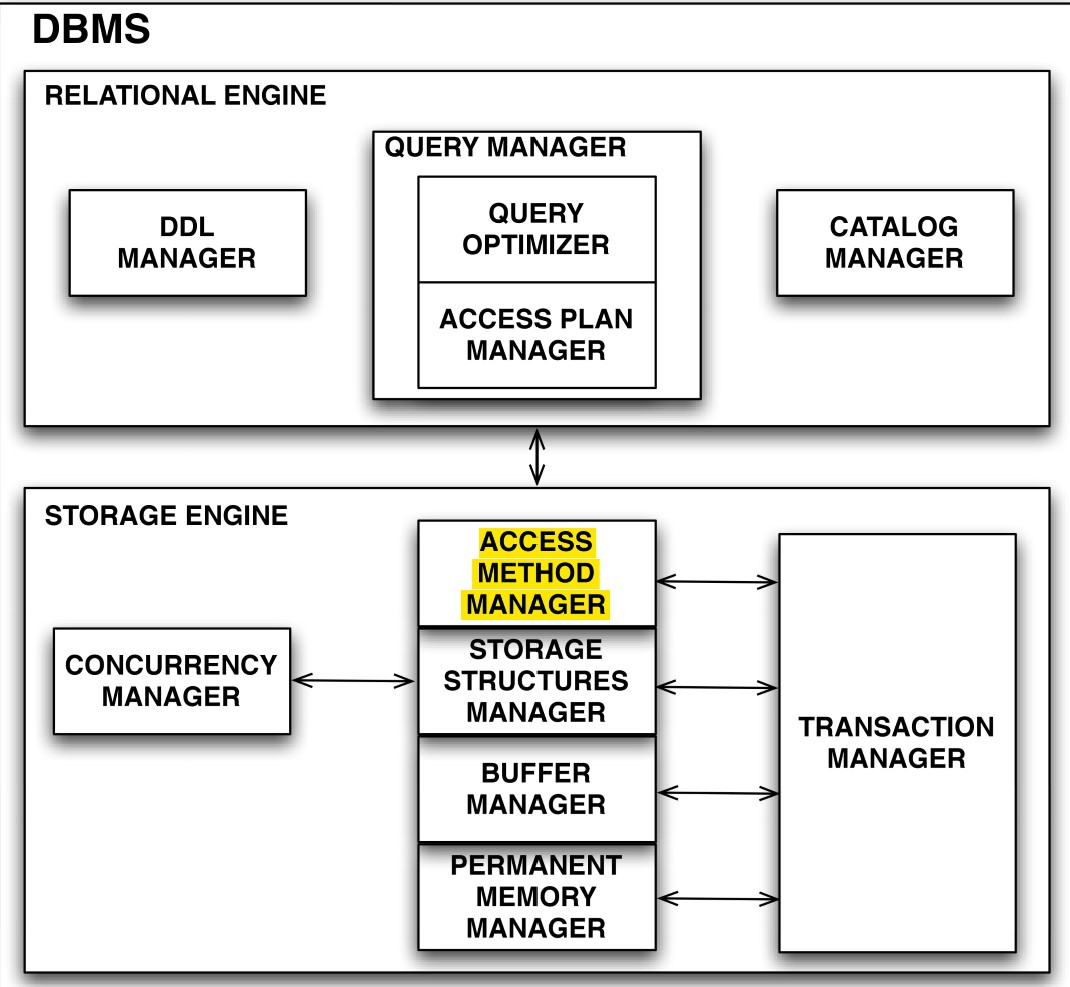
\includegraphics[scale = 0.7]{img/access1.jpg}
		\label{part6}
\end{figure}

\begin{tcolorbox}
The access method manager provides to the relational engine the operators used by its modules to execute the commands for the definition and use of DBs.
\end{tcolorbox}

\subsection{Storage engine}
A DBMS is typically divided into:

\begin{itemize}
    \item the \textbf{relational engine}, which includes modules to support the execution of SQL commands and interacts with the storage engine;
    \item the \textbf{storage engine}, which includes modules to execute the operations on data stored in the permanent memory.
\end{itemize}

Normally, the storage engine is not accessible to the user, who will interact with the relational engine.

While the interface of the relational engine depends on the data model features, the interface of the storage engine depends on the data structures used in permanent memory. To give a better idea of the \textbf{interface of a storage engine}, we will consider the case of the relational system \textbf{JRS}, which stores relations in heap files and provides B+– tree indexes to facilitate data retrieval. The operators on data exported by the storage engine are procedural and can be grouped into the following categories:

\begin{itemize}
    \item operators to create the DBs;
    \item operators to start and end a transaction;
    \item operators on heap file and indexes;
    \item operators about access methods available (= ways of retrieving records from a table) for each relation.
\end{itemize}

We now focus on the operators on DBs, on heap files, on indexes and on the operators about access methods.

\subsection{Operators on DBs}
The operators are:
\begin{itemize}
    \item \textit{createDB}, which creates a DB in the specified path;
    \item \textit{createHeapFile}, which creates an heap file in the DB in the specified path;
    \item \textit{createIndex}, which creates an index on a relation attribute, which could be a key, or on multiple attributes.
\end{itemize}

A DB, an heap file or an index can be deleted using \textit{dropDB}, \textit{dropHeapFile} and \textit{dropIndex}

\subsection{Operators on heap files}
A DB table is stored in a heap file, in which there are operators to insert, delete, retrieve or update records with a specified RID, or to get the number of pages used and the number of the record. A \textbf{table} is a set of records where each record contains the same number of fields. Heap files support the \textit{scan} operation to iterate through the records of a file.

\subsection{Operators on indexes}
An index is a set of records (Value, RID), organized as a B+-tree: the Value is the search key, while RID is the identifier of the record with the search key Value. Any number of indexes can be defined on a relation, and a search key can be multi-attribute. The operators available on indexes are those to insert or delete elements, or to get data about the B+–tree used to store them, such as the number of leaves, minimum and maximum search key Value.

\subsection{Access methods operators}

\begin{tcolorbox}
    The Access Methods Manager provides the operators to transfer data between permanent memory and main memory in order to answer a query on a database. 
\end{tcolorbox}

Permanent data are organized as collections of records, stored in heap files, and indexes are optional auxiliary data structures associated with a collection of records. The operators provided by the Access Methods Manager are used to implement the operators of physical query plans generated by the query optimizer. 

Records of a heap file or of an index are accessed by scans. A \textbf{heap file scan operator} simply reads each record one after the other, while an \textbf{index scan} provides a way to efficiently retrieve the RID of a heap file records with a search by key values in a given range. The records of a heap file can be retrieved by a serial scan or directly using their RID obtained by an index scan with a search condition. A heap file or index scan operation is implemented as an \textbf{iterator}, also called cursor, which is an object with methods that allow a consumer of the operation to get the result one record at a time.

When a heap file iterator is created, it is possible to specify the RID of the first record to return, while for index operators a hey ragne is specified.

\subsection{Example of query execution plan}
Let's consider some examples of programs that use access methods operators of the storage engine to execute simple SQL queries: in particular, the programs show a possible \textbf{query plan} that might be generated by the query optimizer of the relational engine (we will see that the query execution plan does not produce an execution plan of this type, but a physical plan). 

Picture \ref{access2} show the execution plan of the given query using the heap files, while in Picture \ref{access3} we assume that there's an index \textit{idxCity} on the attribute \textit{City} os \textit{Students}. Clearly, the second execution plan is more efficient.

\begin{figure}[h!]
		\centering
		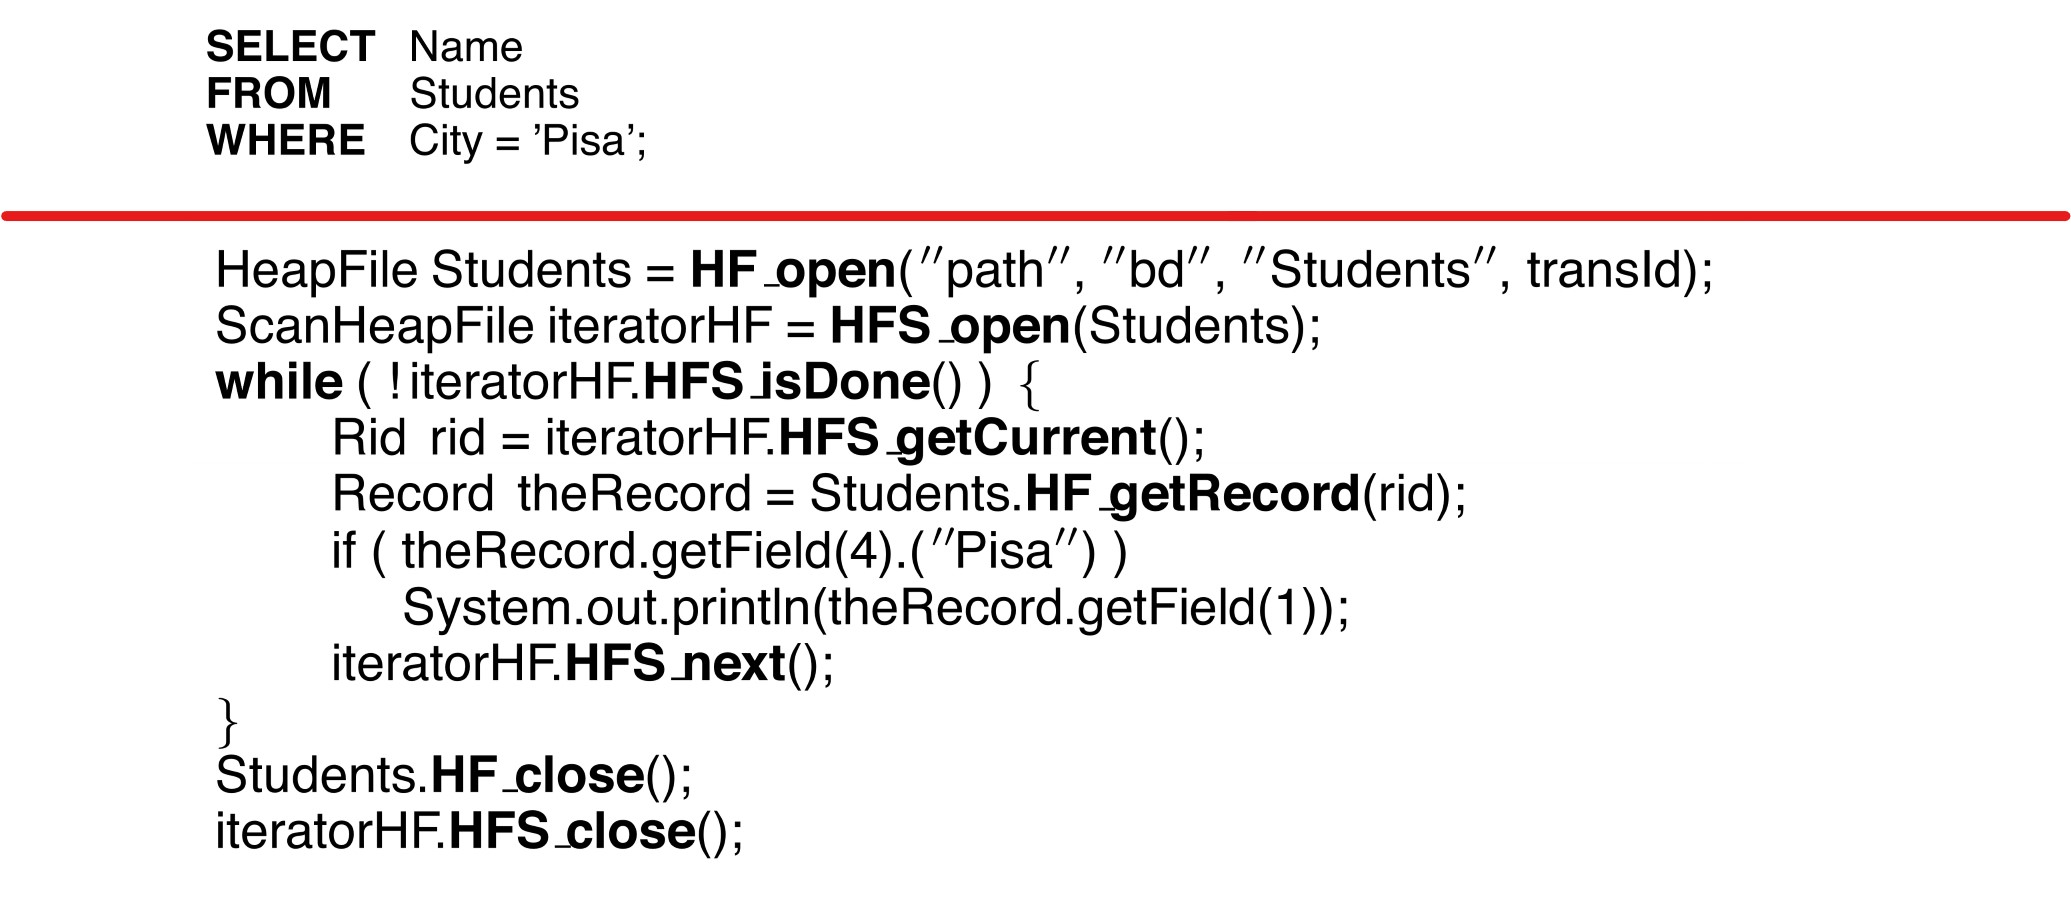
\includegraphics[scale = 0.7]{img/access2.jpg}
		\label{access2}
        \caption{Example of query plan with heap files}
\end{figure}

\begin{figure}[h!]
		\centering
		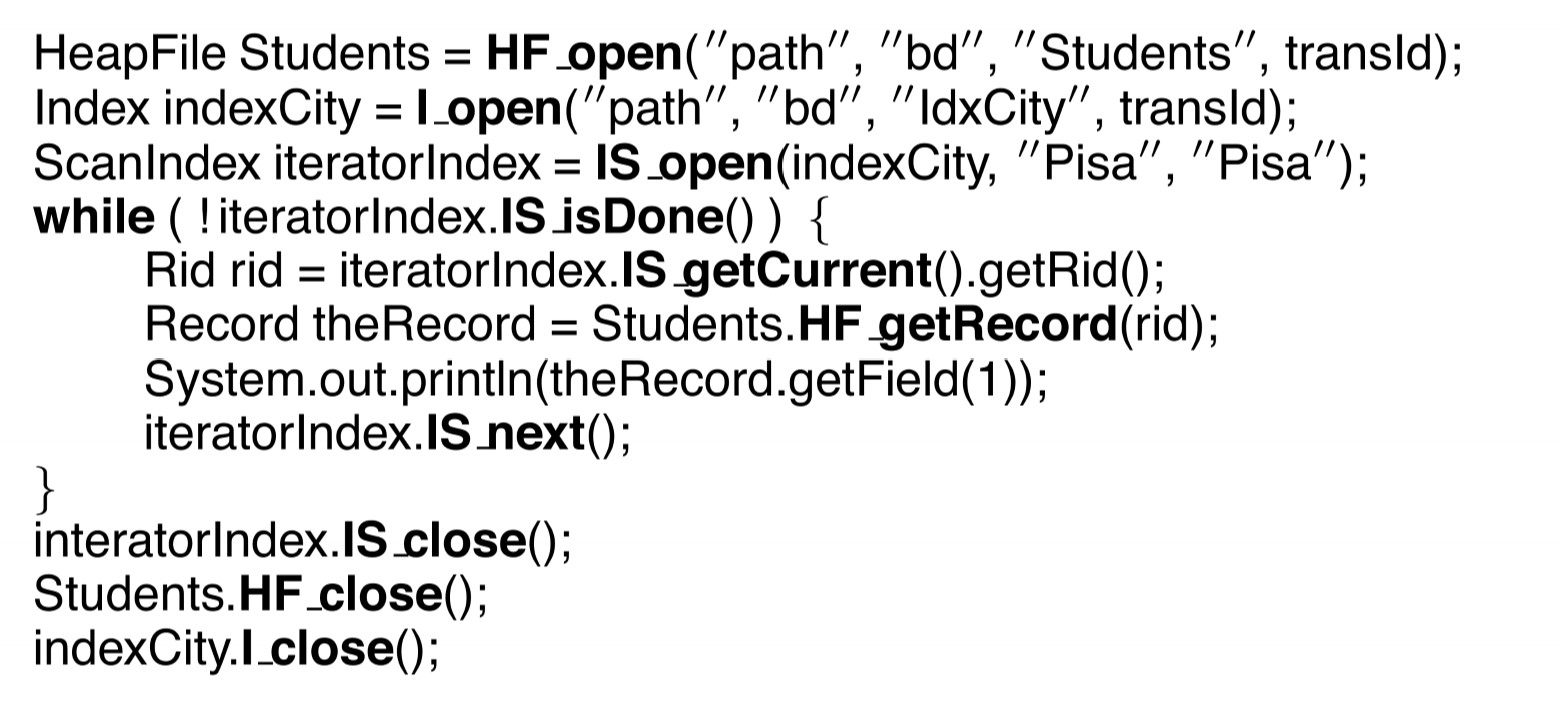
\includegraphics[scale = 0.7]{img/access3.jpg}
		\label{access3}
        \caption{Example of query plan with indexes}
\end{figure}
\section{Implementation of relational operators}

\begin{figure}[h!]
		\centering
		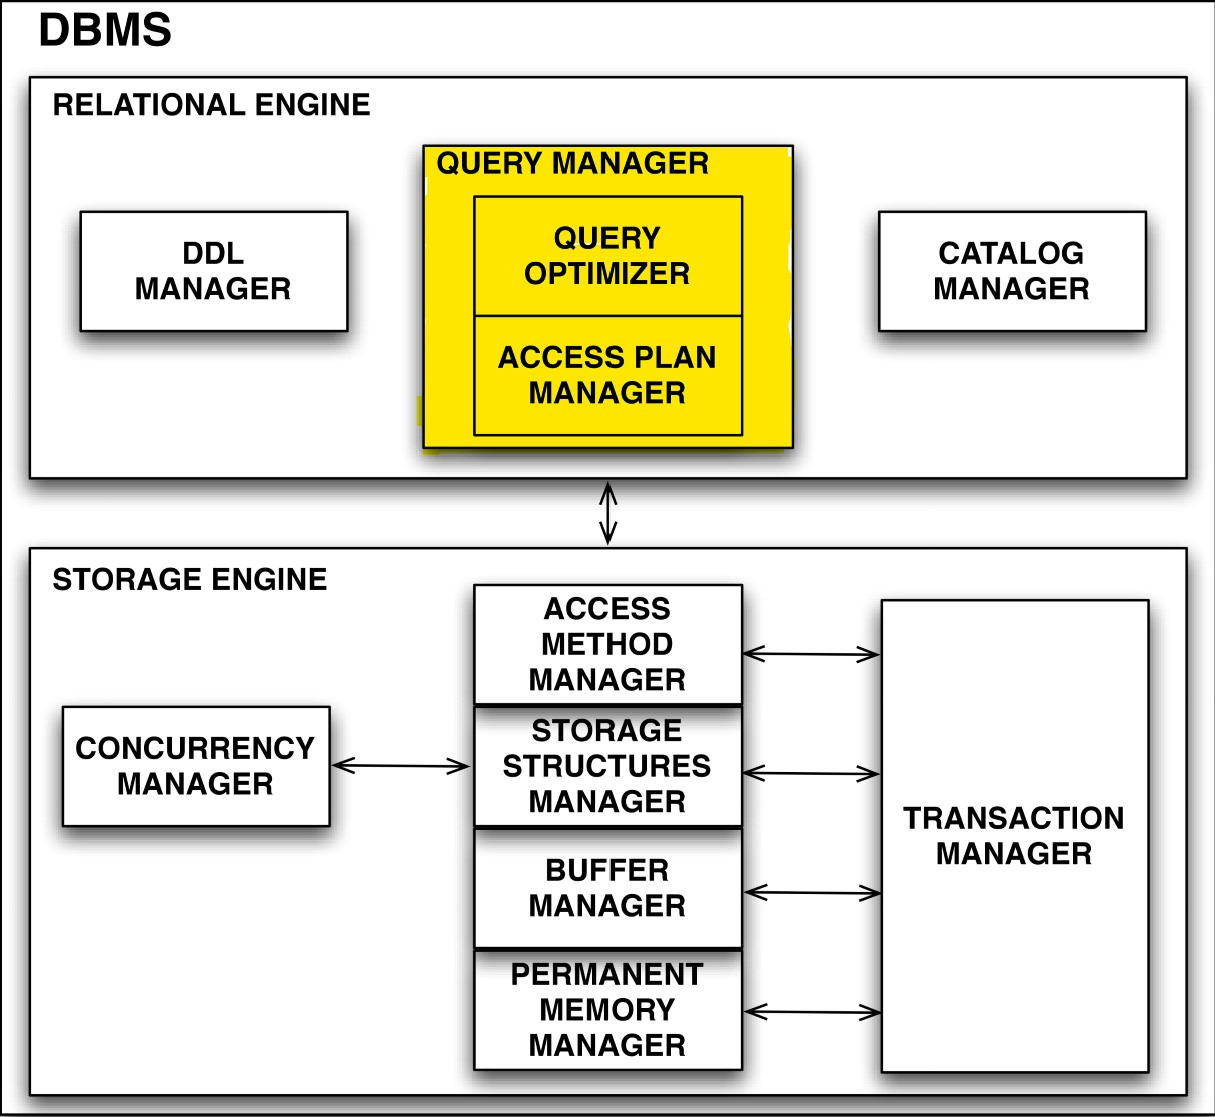
\includegraphics[scale = 0.7]{img/relop1.jpg}
		\label{part6}
\end{figure}

This chapter focuses on the Query Manager, one of the critical components of any DB system, and, in particular, on the algorithms for evaluating relational algebra operations, and how to estimate their cost and size.

\subsection{Assumptions and notation}

\subsubsection{Physical data organization}

\begin{itemize}
    \item each relation has attributes without null values, and it is stored in a heap file, or with the primary organization index sequential. 
    \item to make the operations on relations more efficient, \textbf{indexes} on one or more attributes are used. The indexes are organized as a B+–tree and those for non-key attributes are inverted indexes. We also distinguish two types of indexes:
    \begin{itemize}
        \item a \textbf{clustered index} is built on one or more attributes of a relation sorted on the index key. A relation can only  have one clustered index;
        \item an \textbf{unclustered index} is built on one or more attributes which are not used to sort a relation
    \end{itemize} 
\end{itemize}

\subsubsection{Physical query plan operators}

\begin{tcolorbox}
The \textbf{query optimizer} has the task of determining how to execute a query in an “optimal” way, by considering the physical parameters involved, such as the size of the relations, the data organization and the presence of indexes.
\end{tcolorbox}

 The problem is particularly difficult because, as we will see later, each relational algebra operator can be implemented in different ways and the query optimizer must use appropriate strategies to estimate the costs of the alternatives and choose the one with lowest cost. 
 
 The algorithm chosen by the optimizer to execute a query is represented as a tree, which is called \textbf{physical query plan}. The nodes of this tree are physical operators, each of which is a particular implementation of an operator of the \textbf{relational algebra extended on multisets}. This extension of relational algebra allows to manage multisets, which is what SQL table represent, and for this reason it supports the following operations:

 \begin{itemize}
     \item \textbf{projection with duplicates}: $\pi_X^b(O)$, with $X$ attributes of $O$;
     \item \textbf{duplicate elimination}: $\sigma(O)$;
     \item \textbf{sorting}, used by the SQL statement ORDER BY: $\tau_X(O)$;
     \item \textbf{multiset union, intersection and difference}.
 \end{itemize}

 An example of physical query plan:

 \begin{figure}[h!]
		\centering
		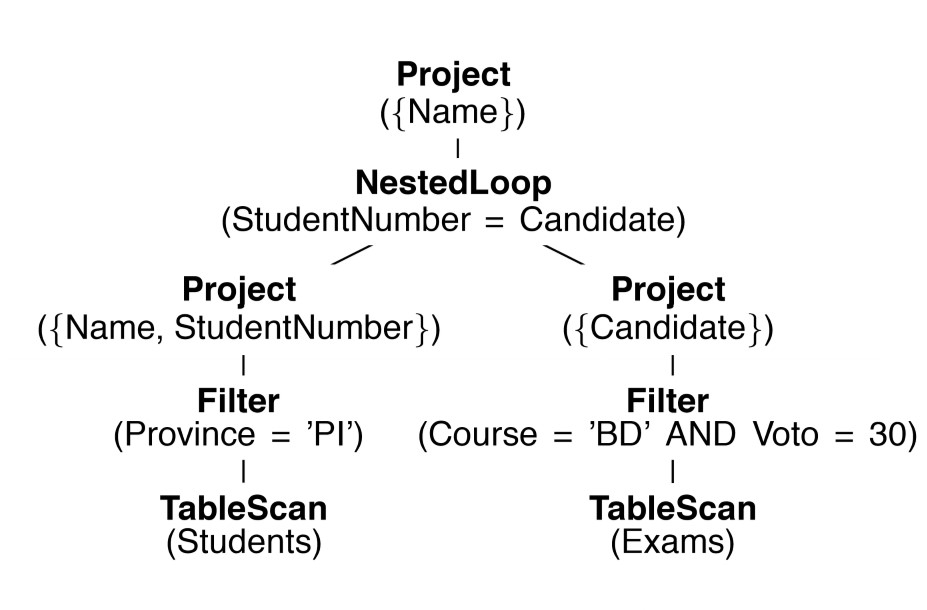
\includegraphics[scale = 0.9]{img/relop2.jpg}
		\label{part6}
\end{figure}

 
Each DBMS has its own \textbf{physical operators} and, for simplicity, we will consider
those of the JRS system. 

\textbf{NOTE}: 
\begin{itemize}
    \item for each physical operator we estimate the data access cost $C$ and the cardinality of its result $E_{rec}$;
    \item physical operators, like the operators of relational algebra, return collections of records with a type that depends on the operator.
\end{itemize} 

\subsubsection{Physical query plan execution}

Physical operators are implemented as \textbf{iterators} that produce the records of the result one at a time on request. An iterator behaves as an object with state, and methods \textit{open}, which initializes the process of getting records, \textit{isDone}, which tests if the iterator has more data to return, \textit{next}, \textit{reset} and \textit{close}.
For example, a physical query plan with root \textit{Plan} is executed as follows:

\begin{figure}[h!]
		\centering
		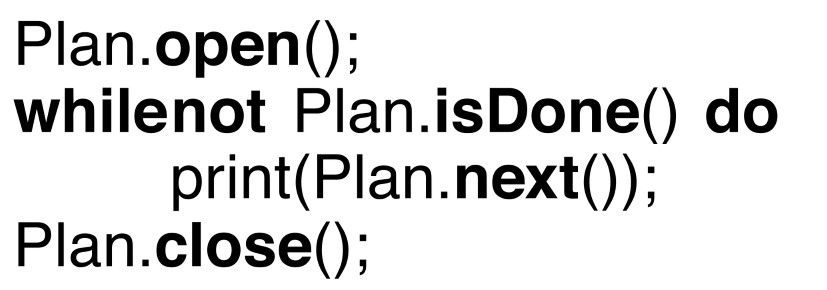
\includegraphics[scale = 0.7]{img/relop3.jpg}
		\label{part6}
\end{figure}

Physical operators are either \textbf{blocking} or \textbf{non-blocking}. A blocking operator, when is opened, must call next exhaustively on its operands before returning its first (or next) record (e.g. the sort operator)

\subsubsection{Cost model}
The \textbf{cost estimate} $C$ of executing a physical operator is given by the number of pages read from or written to the permanent memory to produce the result

\subsection{Physical operators for relation (\textit{R})}
The records of a relation can be retrieved with any of the following operators:

\begin{itemize}
    \item \textbf{TableScan(R)}: it returns the record of $R$ in the order they're stored. This operator belongs to all primary organizations. The cost is:

    $$
    C = N_{\text{pag}(R)}
    $$

    \item \textbf{SortScan(R,A\_i)}: it return the records of $R$ sorted in ascending order according to the attribute $A_i$.
    \begin{itemize}
        \item sorting is done with \textit{merge sort} algorithm
        \item in general, the operator's cost depends on $N_{\text{pag}(R)}$, the number of pages $B$ available in the buffer and the implementation of the \textit{merge sort} algorithm;
        \item this operator is available for all possible primary organizations.
    \end{itemize}
    We assume that the cost is:

    $$
    C = 3N_{\text{pag}(R)}
    $$
    , under the condition that $N_{\text{pag}(R)} < B^2$

    \item \textbf{IndexScan(R,I)}: it returns the records of $R$ sorted in ascending order according to the attribute $A_i$ values of the index $I$. The cost depends both on the type of index and on the type of attribute on which it is defined:

    $$
    C = \begin{cases}
        N_{\text{leaf}}(I) + N_{\text{pag}(R)} & \mbox{if} \text{ I is clustered} \\
        N_{\text{leaf}}(I) + N_{\text{rec}(R)} & \mbox{if} \text{ I is unclustered} \\
        N_{\text{leaf}}(I) + \ceil*{N_{\text{key}}(I) \times \phi (\ceil*{N_{\text{rec}}(R)/N_{\text{key}}(I)}, N_{\text{pag}(R))}} & \mbox{if} \text{ I is an inverted index}
        \end{cases}
    $$

    Note that $N_{\text{leaf}}(I)$ represents the cost of accessing the index, while the other addend represents the cost for accessing the data, and it depends on the nature of the index $I$.

    \item \textbf{IndexSequentialScan(R,I)}: it returns the records of $R$, stored with primary organization \textit{index sequential I}, sorted in ascending order on the primary key values. The cost is:

    $$
    C = N_{\text{leaf}}(I)
    $$
    
\end{itemize}

\textbf{NOTE}: in all the cases, the cardinality of the result is:

$$
E_{\text{rec}} = N_{\text{rec}(R)}
$$

\subsection{Physical operator for projection with duplicates ($\pi^b$)}

\begin{itemize}
    \item \textbf{Project(O,A\_i)}: it returns the records of the projections of the records of $O$ over the attributes ${A_i}$. The cost is:

    $$
    C = C(O)
    $$
    , if there are no subqueries.

    The cardinality of the result is:

    $$
    E_{\text{rec}} = E_{\text{rec}(O)}
    $$

    This operator is always available.

    \item \textbf{IndexOnlyScan(R,I,A\_i)}: it returns the sorted records of $\pi_{A_i}^b(R)$ by using the index $I$ on the attributes $A_i$. The cost is:

    $$
    C = N_{\text{leaf}}(I)
    $$

    , while the cardinality of the result is:

    $$
    E_{\text{rec}} = N_{\text{rec}(R)}
    $$
    
\end{itemize}

\subsection{Physical operators for duplicate elimination ($\delta$)}

\begin{itemize}
    \item \textbf{Distinct(O)}: returns the record of $O$ sorted and without duplicates, i.e. it converts $O$ from a multiset to a set. The crucial precondition is that the records of $O$ are sorted. The cost is:

    $$
    C = C(O)
    $$

    \item \textbf{HashDistinct(O)}: it eliminates the duplicates of $O$ using an hash technique. Suppose that we have $B + 1$ pages in the buffer to perform duplicate elimination, then this technique is composed of two phases that use two different hash functions:
    
    \begin{itemize}
        \item the \textit{partitioning phase}, in which the first hash function $h_i$ is applied to each record of $O$ to distribute the records uniformly in the $B$ pages: the result are $B$ files, each containing a collection of records with the same hash value;
        \item the \textit{duplicate elimination phase}, in which the second hash function $h_2$ is applied to all record attributes of each page of each partition in order to eliminate the duplicates.
    \end{itemize}

    The cost is:

    $$
    C = C(O) + 2 \times N_{\text{pag}(O)}
    $$
    
\end{itemize}

We notice that the \textit{HashDistinct} technique has the same cost of the \textit{Distinct} tecnhique with the sorting of the operand records, but it does not procude a sorted result.

\subsection{Physical operators for selection ($\sigma$)}

\begin{itemize}
    \item \textbf{Filter(O, $\psi$)}: it returns the records of $O$ satisfying the condition $\psi$. The cost is:

    $$
    C = C(O)
    $$

    This operator is always available.

    \item \textbf{IndexFilter(R,I,$\psi$)}: it returns the records of $R$ satisfying the condition $\psi$ with the use of the index $I$, defined on attributes $\psi$ ; more specifically:
    \begin{itemize}
        \item it uses the index to find the sorted set of RIDs satisfying the condition, using \textbf{RIDIndexFilter(I, $\psi$)};
        \item retrieves the records of $R$ using \textbf{TableAccess(O,R)}.
    \end{itemize}

    The cost is given by:

    $$
    C = C_I + C_D
    $$
    , where $C_I$ and $C_D$ depend on the type of index and the type of attributes on which it is defined.

    \item \textbf{IndexSequentialFilter(R,I,$\psi$)}: it returns the sorted records of $R$, stored with the primary organization \textit{index sequential I}, satisfying the condition $\psi$. The cost is:

    $$
    C = \ceil*{s_f(\psi) \times N_{\text{leaf}()I}}
    $$

    \item \textbf{IndexOnlyFilte(R,I,$A_i$,$\psi$)r}: it returns the sorted records of $\pi_{A_i}^b(\sigma_{\psi}(R))$, using only the index I. The cost is:

    $$
    C = \ceil*{s_f(\psi) \times N_{\text{leaf}()I}}
    $$

    \item \textbf{OrIndexFilter(R,{$I_i$,$\psi_i$ })}: it returns the records of $R$ satisfying the disjunctive condition $\psi = \psi_1 \lor \psi_2 \lor ... \lor \psi_n$ using the index $I_i$ for each $\psi_i$. More specifically:
    \begin{itemize}
        \item it uses the index to find a sorted union of the RID lists of records matching each terms $\psi_i$;
        \item retrieves the records of $R$.
    \end{itemize}
    The cost is:

    $$
    C = C_I + C_D
    $$
    , where 

    $$
    C_I = \ceil*{\sum\limits_{k = 1}^n C_I^k }
    $$

    and 

    $$
    C_D = \ceil*{\Phi (E_{\text{rec}} , N_{\text{pag}}(R))}
    $$

    \item \textbf{AndIndexFilter(R,{ $I_i$, $\psi_i$ })}: it returns the records of $R$ satisfying the conjunctive condition $\psi = \psi_1 \land \psi_2 \land ... \land \psi_n$ using the index $I_i$ for each $\psi_i$. More specifically:
    \begin{itemize}
        \item it uses the index to find a sorted intersection of the RID lists of records matching each terms $\psi_i$;
        \item retrieves the records of $R$.
    \end{itemize}
    The cost is:

    $$
    C = C_I + C_D
    $$
    , where 

    $$
    C_I = \ceil*{\sum\limits_{k = 1}^n C_I^k }
    $$

    and 

    $$
    C_D = \ceil*{\Phi (E_{\text{rec}} , N_{\text{pag}}(R))}
    $$
    
\end{itemize}

Picture \ref{relop4} and \ref{relop5} show two examples of access plans that are constructed from two simple queries: note that in the second query we can use IndexFilter because there's an index on the attribute $A$ and , but we cannot use IndexOnlyFilter because we have "SELECT *".

\begin{figure}[h!]
		\centering
		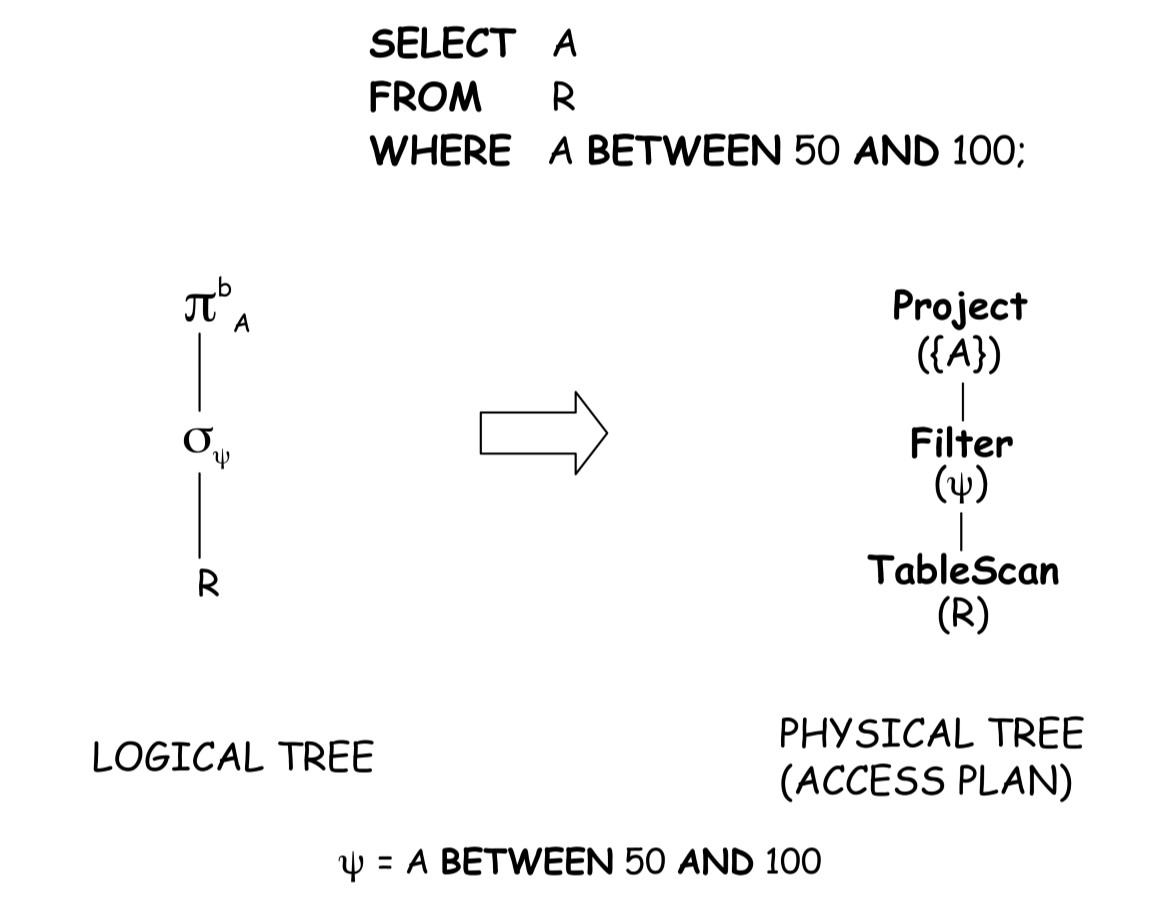
\includegraphics[scale = 0.7]{img/relop4.jpg}
		\label{relop4}
\end{figure}

\begin{figure}[h!]
		\centering
		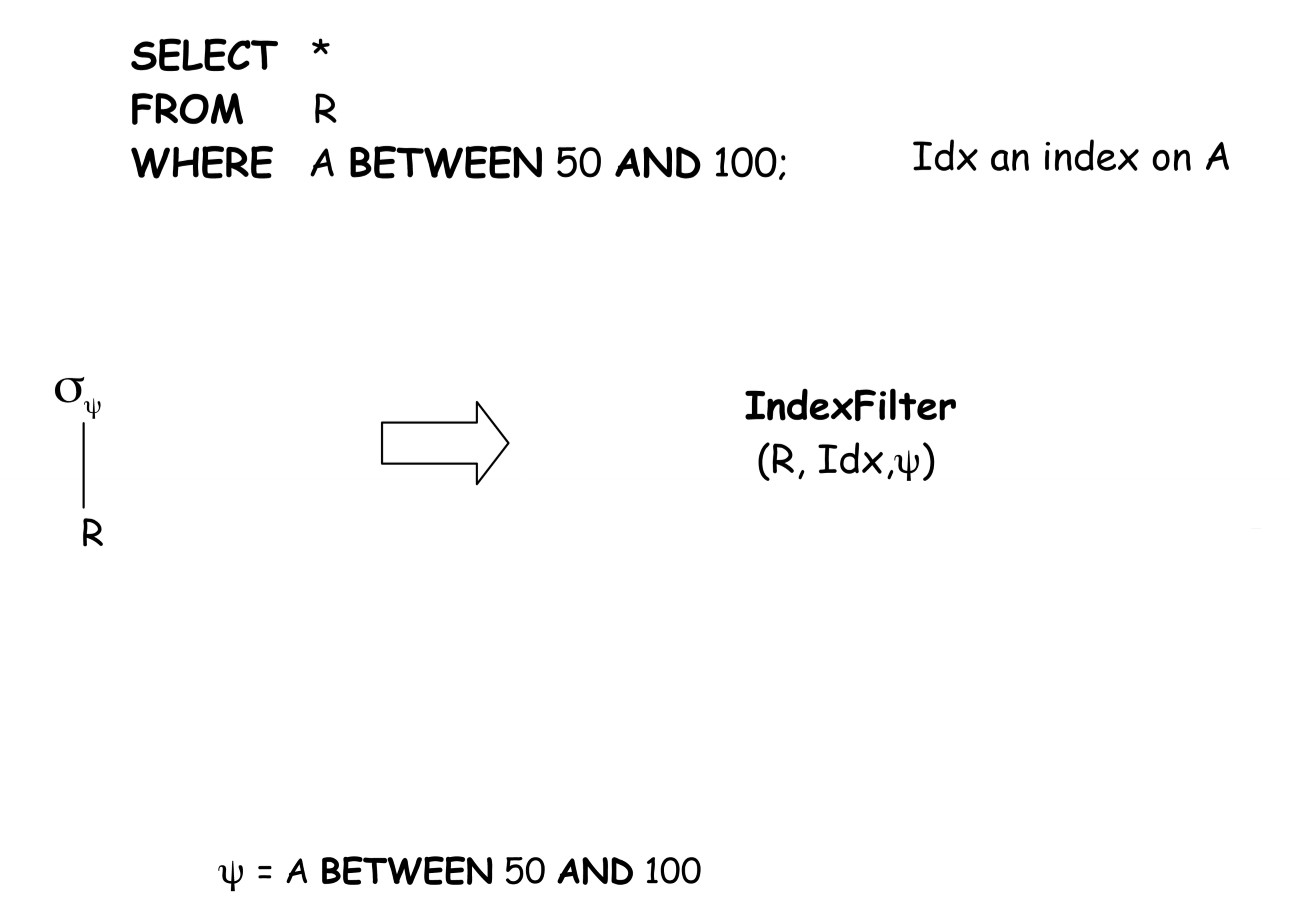
\includegraphics[scale = 0.7]{img/relop5.jpg}
		\label{relop5}
\end{figure}


\subsection{Physical operators for grouping ($\gamma$)}
The records of $R$ are partitioned according to their values in one set of attributes $A_i$, called the \textit{grouping attributes}. Then, for each group, the values in certain other attributes are aggregated with the functions $f_i$. The result of this operation is one record for each group. 
To execute the grouping of the operand $O$ result, the following physical operators are used, which differ in the way the records of $O$ are partitioned:

\begin{itemize}
    \item \textbf{GroupBy(O,$A_i$,${f_i}$)}: the records of $O$ are sorted on the grouping attributes $A\_i$, so that the records of each group are next to each other. Note that in the set ${f_i}$ there are the aggregation functions present in the SELECT and HAVING clauses. The cost is:

    $$
    C = C(O)
    $$

    \item \textbf{HashGroupBy(O,${A_i}$,${f_i}$)}: the records of $O$ are partitioned using an hash function on the attributes ${A_i}$:
    
    \begin{itemize}
        \item \textit{partitioning phase}: using the hash function $h_1$, a partition is created;
        \item \textit{grouping phase}: using the hash function $h_2$ to all grouping attributes, the records of each partition are grouped.
    \end{itemize}
    
    The cost is:

    $$
    C = C(O) + 2 \times N_{\text{pag}(O)}
    $$
    
\end{itemize}

Picture \ref{relop6} shows an example of GROUP BY query that is transformed into an access plan.


\begin{figure}[h!]
		\centering
		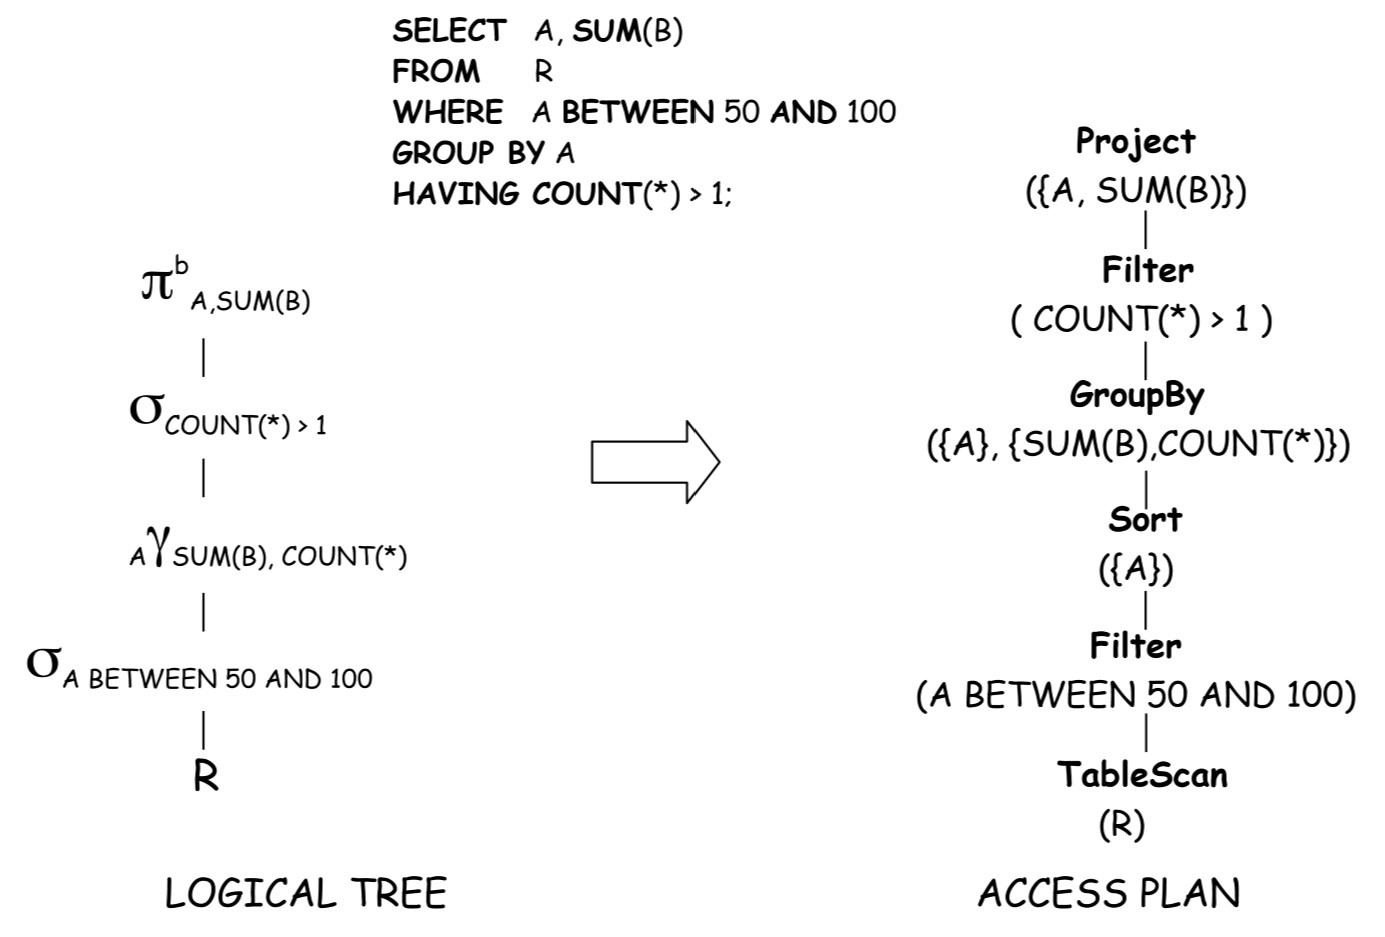
\includegraphics[scale = 0.8]{img/relop6.jpg}
		\label{relop6}
\end{figure}

\subsection{Physical operators for join ($\bowtie$)}
The JOIN operation can be considered as cartesian product + filter operation: the cartesian product crates all the possible pairs, while the filter operation removes the pairs in which the primary key does not match. However, if we have two sets $A$ and $B$, then the number of pairs is  $|A \times B|$, and most of them are discarded, so it is an inefficient operation. For this reason, the two possible options to optimize the JOIN operation is:

\begin{itemize}
    \item reduce the number of candidates using an index;
    \item reduce the cost of access, using the same number of candidates.
\end{itemize}

We only consider $O_E \bowtie_{\psi_J} O_I$, where:
\begin{itemize}
    \item $O_E$ is the external operand;
    \item $O_I$ is the internal operand;
    \item $\psi_J$ is the join condition.
\end{itemize}

\begin{itemize}
    \item \textbf{NestedLoop($O_E$, $O_I$ $\psi_J$)}:

    \begin{figure}[h!]
		\centering
		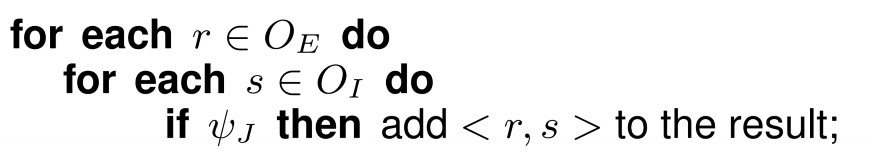
\includegraphics[scale = 0.8]{img/relop7.jpg}
		\label{relop6}
    \end{figure}

    The cost is:

    $$
    C = C(O_E) + E_{\text{rec}(O_E)} \times C(O_I)
    $$
    , but the order of the loops matter! From the cost function we can see that all the pages of the internal operand are accessed for each page of the external operand, so it is more convenient to have as external operand the relation with more tuples.

    \item \textbf{PageNestedLoop($O_E$, $O_I$, $\psi_J$)}: this operator exploit the buffer in order to reduce the number of disk accesses: in particular, the result of $O_I$ is scanned once per page of $O_E$, instead of per each record of $O_E$. For this reason, the larger the page size, the better in terms of computational complexity.

    \begin{figure}[h!]
		\centering
		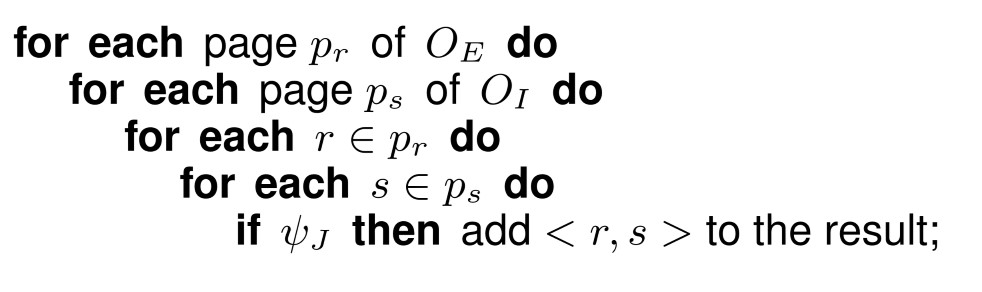
\includegraphics[scale = 0.8]{img/relop8.jpg}
		\label{relop6}
    \end{figure}

    The cost is:

    $$
    C = C(O_E) + N_{\text{pag}(O_E)} \times C(O_I)
    $$

    In this case, the algorithm cost is lower when the external relation is the one with fewest pages.
    
\end{itemize}

\textbf{NOTE}:
\begin{itemize}
    \item both NestedLoop and PageNestedLoop do not have any knowledge about the predicates, so no index is used;
    \item PageNestedLoop is better than NestedLoop, being $N_{\text{pag}(O_E)} < N_{\text{rec}(R)}$, but it does not produce a sorted result.
\end{itemize}

\begin{itemize}
    \item \textbf{IndexNestedLoop($O_E$, $O_I$, $\psi_J$)}: in this case we have some knowledge about the predicates, in particular we can use an index in order to filter the records and reduce the number of candidates. However, the preconditions are:
    \begin{itemize}
        \item the join is an \textit{equi-join}. It can be used not only for equi-join, provided that it has an access method for the predicate;
        \item there is an IndexFilter on the internal operand.
    \end{itemize}

    \begin{figure}[h!]
		\centering
		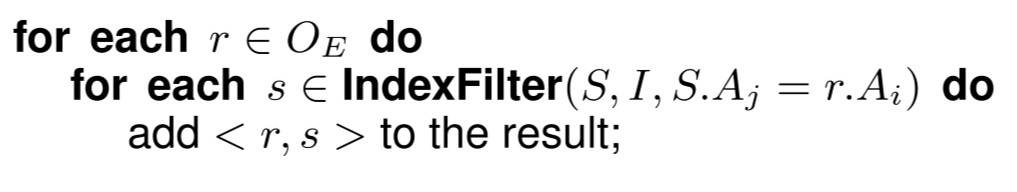
\includegraphics[scale = 0.8]{img/relop9.jpg}
		\label{relop6}
    \end{figure}

    The cost is:

    $$
    C = C(O_E) + E_{\text{rec}(O_E)} \times (C_I + C_D)
    $$
    , where $(C_I +C_D)$ is the cost to retrieve the matching records of $S$ with a record of $O_E$ that depends on the index type.

    \item \textbf{MergeJoin($O_E$, $O_I$, $\psi_J$)}: in this case the precondition are:

    \begin{itemize}
        \item the join is an \textit{equi-join};
        \item $O_E$ and $O_I$ are sorted on the join attributes $O_E.A_i$ and $O_I.A_i$;
        \item the join attribute $O_E.A_i$ is a key.
    \end{itemize}

    The cost is:

    $$
    C = C(O_E) + C(O_I)
    $$

    This operator is efficient provided that $O_E$ and $O_I$ are sorted, otherwise we have to consider some additional costs.

    \item \textbf{HashJoin($O_E$, $O_I$, $\psi_J$)}: similarly to HashDisinct and HashGroupBy, this operator computes the join in two phases:
    \begin{itemize}
        \item in the \textit{partitioning phase}, the records of $O_E$ and $O_I$ are partitioned using the first hash function $h_1$ applied to the join attributes. If two tuples are joined, they belong to the same partition but in different pages.

        \begin{figure}[H]
		\centering
		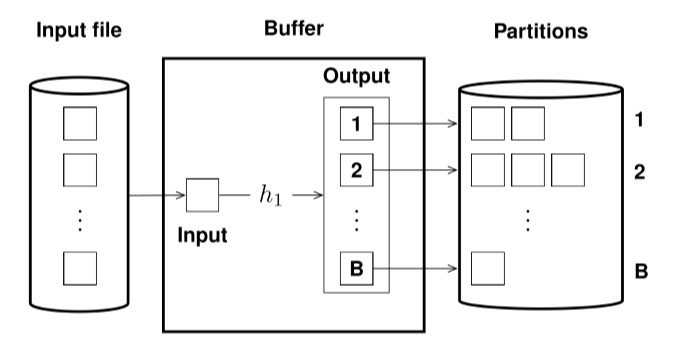
\includegraphics[scale = 0.8]{img/relop10.jpg}
		\label{relop6}
        \end{figure}

        
        \item in the \textit{probing phase}, for each partition $B_i$ 
        \begin{itemize}
            \item the records of $O_E$ are read and inserted into buffer hash table with $B$ pages using the function $h_2$ applied to the join attribute values;
            \item the records of $O_I$ are read one page at a time, and which of them join with those of $O_E$ is checked with $h_2$, and they're added to the result;
        \end{itemize}

        \begin{figure}[H]
		\centering
		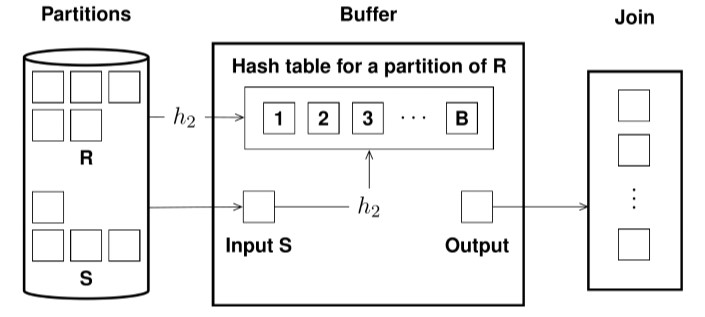
\includegraphics[scale = 0.9]{img/relop11.jpg}
		\label{relop6}
        \end{figure}

    \end{itemize}

    The costs are:

    $$
    C_{\text{partitioning}} = C(O_E) + C(O_I) + N_{\text{pag}(O_E)} + N_{\text{pag}(O_I)}
    $$

    $$
    C_{\text{probing}} = N_{\text{pag}(O_E)} + N_{\text{pag}(O_I)}
    $$

    , so the total cost is:

    $$
    C = C(O_E) + C(O_I) + 2 \times (N_{\text{pag}(O_E)} + N_{\text{pag}(O_I))}
    $$
    
\end{itemize}

In general, since $O_E \bowtie_{\psi_J} O_I = \sigma_{\psi_J}(R \times S)$, the \textbf{cardinality of the result} is :

$$
E_{\text{rec}} = \ceil*{s_f(\psi_J) \times E_{\text{rec}(O_E)} \times E_{\text{rec} (O_I) }  }
$$

Pictures \ref{relop12} and \ref{relop13} show two examples of join queries that are trasformed into access plans.

\begin{figure}[h!]
		\centering
		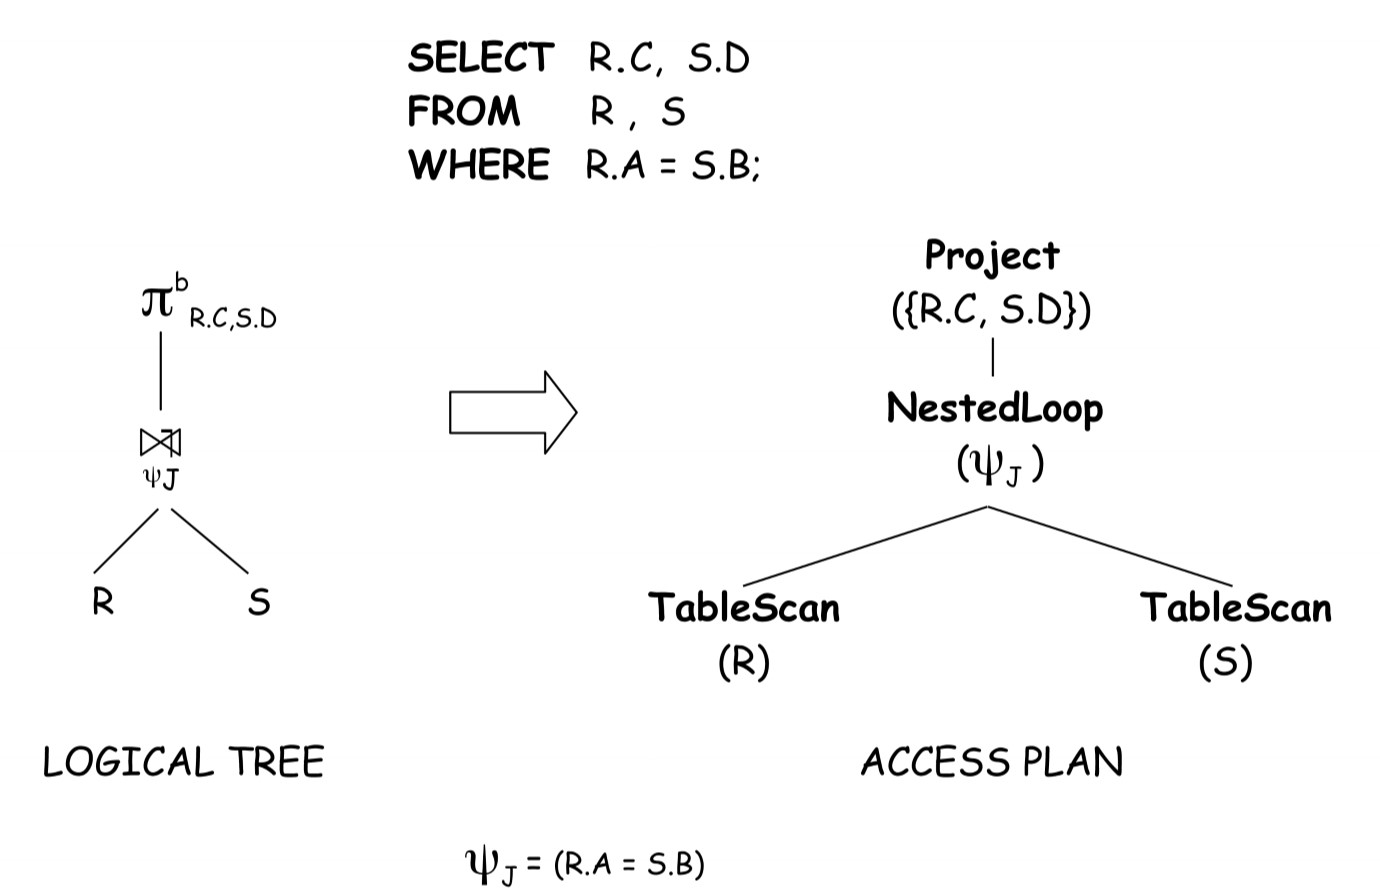
\includegraphics[scale = 0.7]{img/relop12.jpg}
		\label{relop12}
\end{figure}


\begin{figure}[h!]
		\centering
		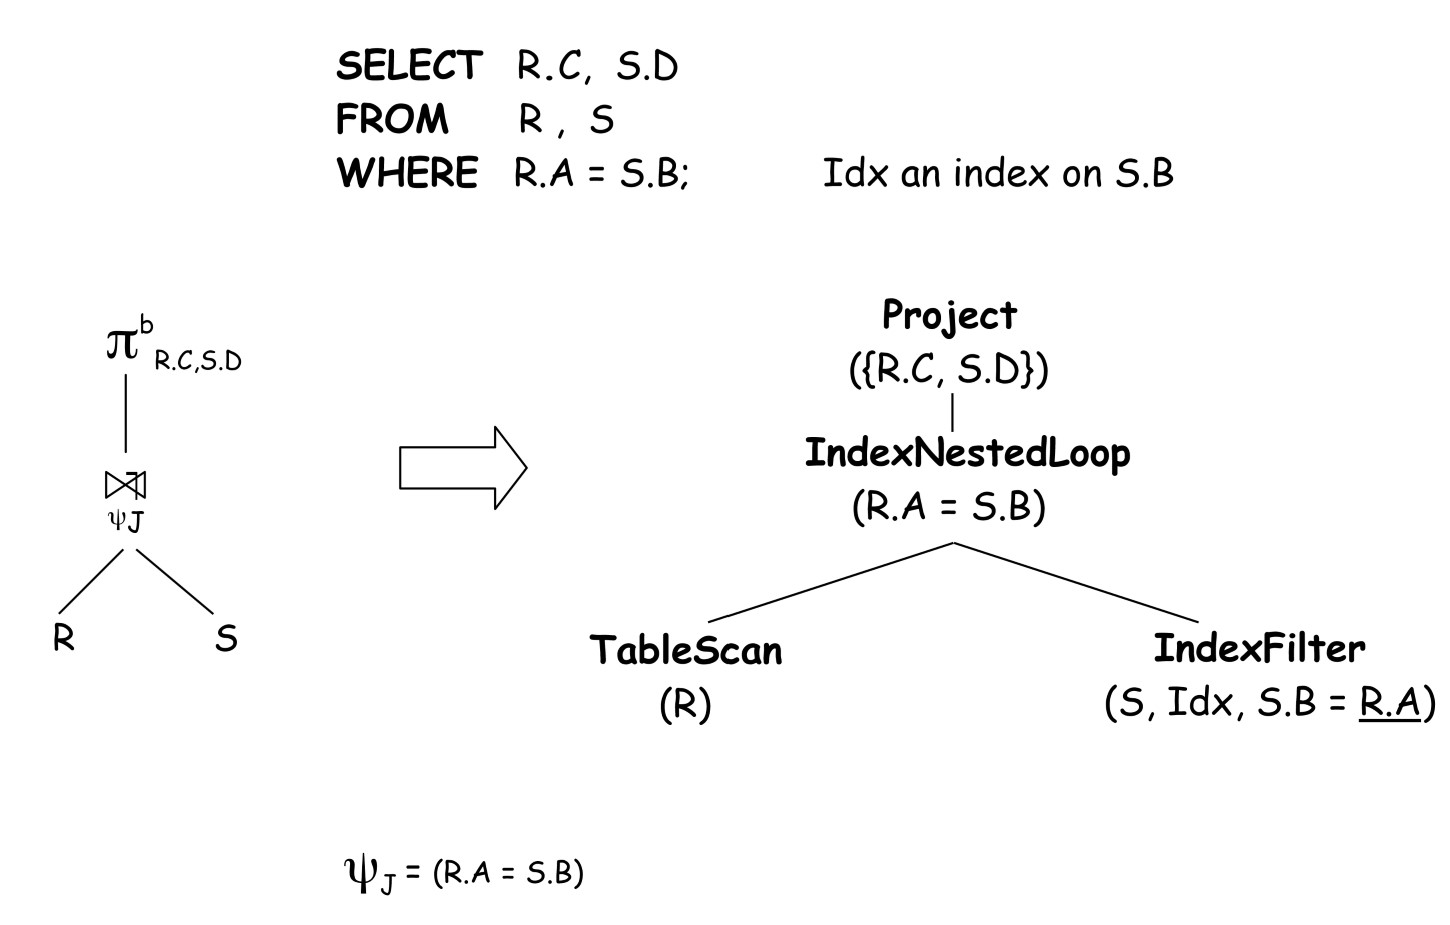
\includegraphics[scale = 0.7]{img/relop13.jpg}
		\label{relop13}
\end{figure}

\subsection{Physical operators for set and multiset operations}

\begin{itemize}
    \item \textbf{Union($O_E$,$O_I$)}, \textbf{Except($O_E$,$O_I$)} and \textbf{Intersect($O_E$,$O_I$)} require that the operand are sorted and do not have any duplicate element. In this case the cost is:

    $$
    C = C(O_E) + C(O_I)
    $$

    \item \textbf{UnionAll($O_E$,$O_I$)}, \textbf{ExceptAll($O_E$,$O_I$)} and \textbf{IntersectAll($O_E$,$O_I$)} do not eliminate duplicates, so they implement the multiset operations. The cost is:

    $$
    C = C(O_E) + C(O_I)
    $$
    
\end{itemize}
\section{Query optimization}

\begin{figure}[h!]
		\centering
		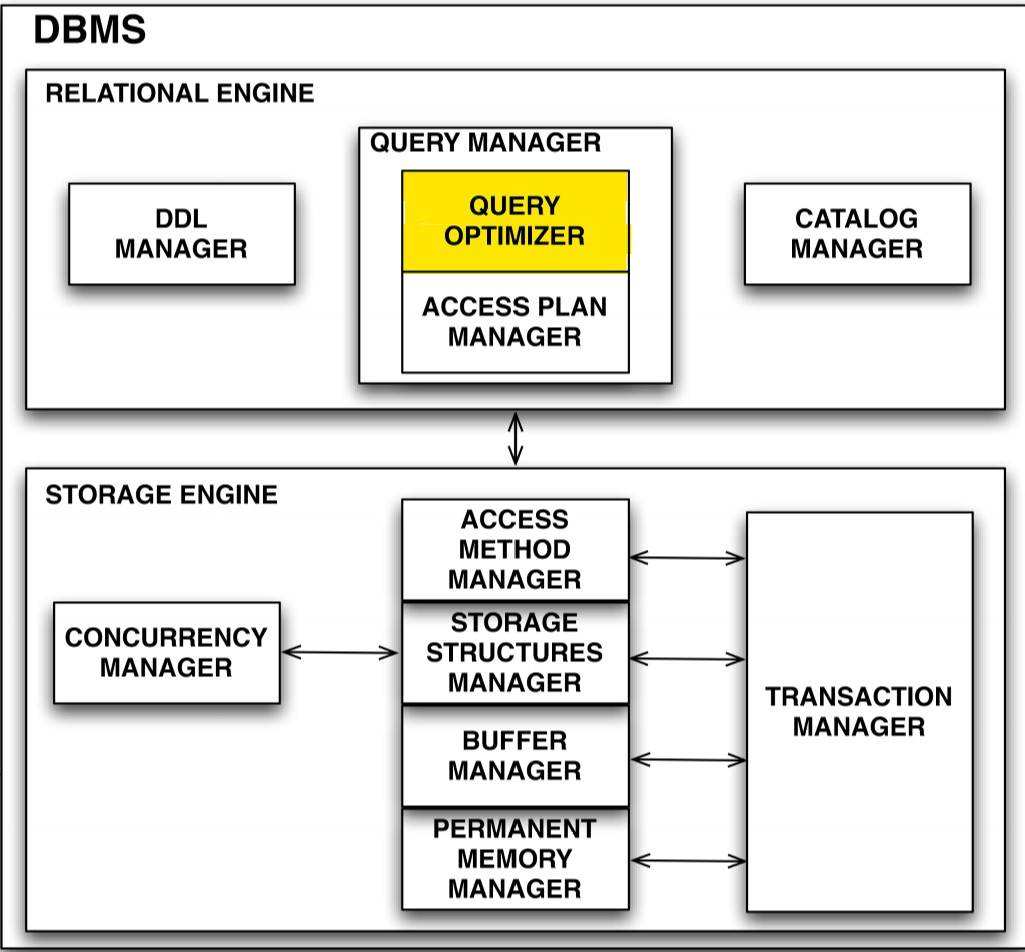
\includegraphics[scale = 0.7]{img/queop1.jpg}
		\label{relop13}
\end{figure}

In this chapter the focus is on query processing and on how to find the best plan to execute a query. In particular, we study the optimizer organization, a fundamental component of the \textbf{Query Manager}, which selects the optimal physical plan to execute queries using the operators and data structures of the Storage Engine. We will also show how functional dependencies, well known for relational schema design, are also important for query optimization.

\subsection{Introduction}
The \textbf{goal} of the optimizer is to find an efficient plan to execute a query. This problem is complex because:

\begin{itemize}
    \item a query can be written in several equivalent ways;
    \item a relational algebra operator can be implemented with different physical operators.
\end{itemize}

, so the optimizer will use some heuristic methods to find a good solution quickly.

The optimization can be:
\begin{itemize}
    \item \textbf{dynamic}, i.e. the physical plan is generated at run time when the query is executed, taking into account some informations about the DB and the available data structures;
    \item \textbf{static}, i.e. the physical plan in generated at the program compilation time
\end{itemize}

\subsubsection{Query processing phases}
\begin{enumerate}
    \item \textbf{query analysis}: the correctness of the SQL query is checked and it is transformed into relational algebra, i.e. the \textit{initial logical query plan}
    \item \textbf{query transformation}: the initial logical plan is transformed into an equivalent one that provides a better query performance
    \item \textbf{physical plan generation}: alternative algorithms for the query execution are considered and the \textit{physical query plan} with the lowest cost is chosen. This step makes query processing hard, because there's a large number of alternative solutions to consider in order to choose the best one
    \item \textbf{query evaluation}: the physical plan is executed
\end{enumerate}

\subsection{Query analysis phase}
\begin{enumerate}
    \item lexical and syntax query analysis
    \item semantic query analysis, in which the system check both the query semantic correctness and that the user has appropriate privileges
    \item simplification of the \textbf{WHERE} condition using:
    \begin{itemize}
        \item equivalence rules of boolean expressions;
        \item elimination of contradictory conditions;
        \item elimination of NOT conditions;
    \end{itemize}
    \item generation of the internal representation of the query as an \textbf{initial logical query plan}, represented as an expression tree of relational algebra operations. For example, the query: 

    \begin{figure}[h!]
		\centering
		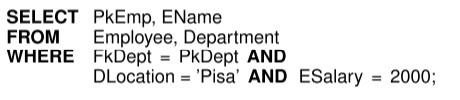
\includegraphics[scale = 1.3]{img/queop2.jpg}
		\label{relop13}
    \end{figure}

    is transformed into the following logical plan:

    \begin{figure}[h!]
		\centering
		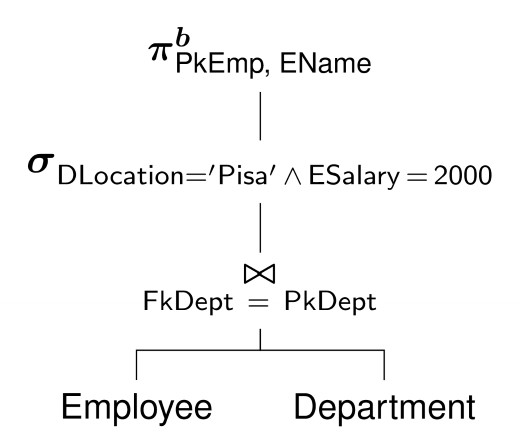
\includegraphics[scale = 0.9]{img/queop3.jpg}
		\label{queop3}
        \caption{Initial logical query plan}
    \end{figure}
    
\end{enumerate}

\subsection{Query transformation phase}
In this phase, the \textit{initial logical query plan} is transformed into an equivalent one using a set of equivalence rules, for example the \textit{cascading of selections} or the \textit{commutativity of selection and projection}. In general, the following rules are followed:

\begin{itemize}
    \item selections are pushed below projections and they're grouped;
    \item selections and projections are pushed below joins;
    \item unnecessary projections are deleted;
    \item projections are grouped.
\end{itemize}

Picture \ref{queop4} shows an example of transformation of the initial logical query plan of Picture \ref{queop3}.

\begin{figure}[h!]
		\centering
		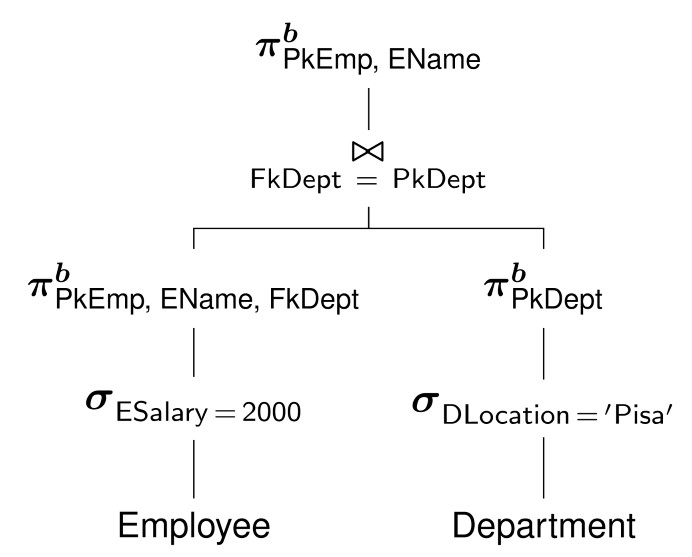
\includegraphics[scale = 0.9]{img/queop4.jpg}
		\label{queop4}
        \caption{Transformation of the initial logical query plan}
\end{figure}

\subsubsection{DISTINCT elimination}
The DISTINCT operation requires SORT, which is costly, so we use the functional dependencies theory to discover if an interesting functional dependency can be inferred into the result of a query. In general, let $A$ be the set of attributes of the result and $K$ be the union of the attributes of the key of every table used in the query, then if $A -> K$, then the operator $\delta$ for duplicate elimination is unnecessary.

\subsubsection{GROUP BY elimination}
As DISTINCT, also GROUP BY requires the SORT operation. In this case, the elimination can happen:
\begin{itemize}
    \item if there's only a single group;
    \item each group is composed of a single tuple
\end{itemize}

\subsubsection{WHERE-subquery elimination}
In general, to execute such queries, the optimizer generate a physical plan for the subquery, which then will be executed for each record processed by the outer query. Therefore, the presence of a \textbf{subquery} makes the \textbf{physical plan more expensive}, and for this reason techniques have been studied to transform a query into an equivalent one without the subquery, which the optimizer processes more efficiently. In particular, all the subqueries can be rewritten using EXISTS and NOT EXISTS, and in certain cases they can be eliminated with the introduction of JOIN.

\begin{figure}[h!]
		\centering
		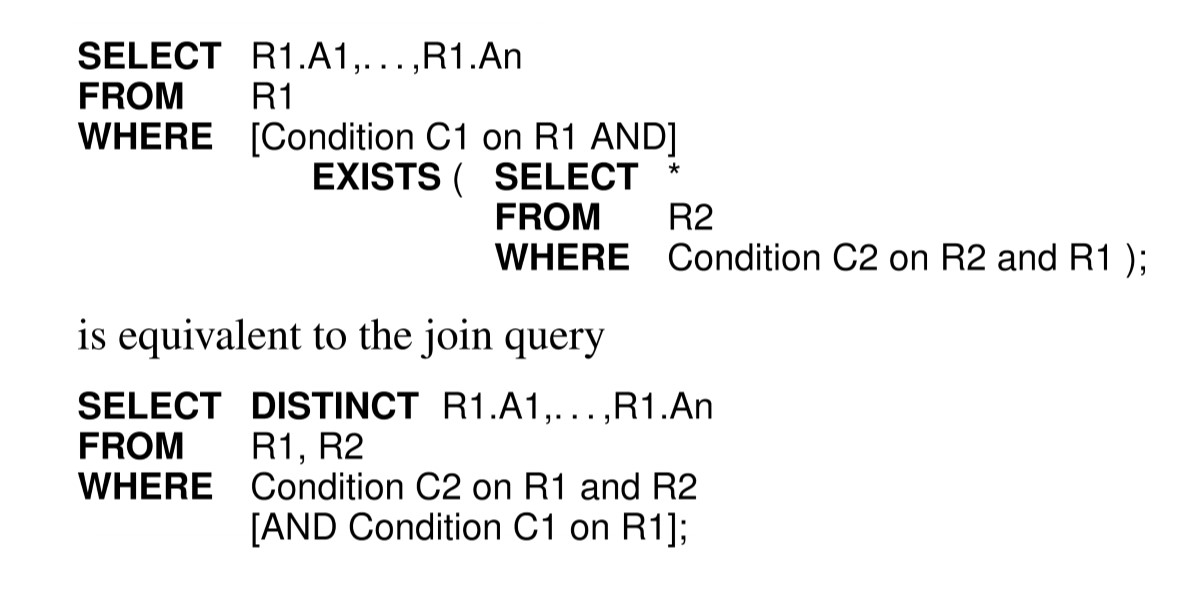
\includegraphics[scale = 0.9]{img/queop5.jpg}
		\label{queop4}
\end{figure}

\textbf{NOTE}: by using the join we create all the possible pairs, so we must check for DISTINCT!

Complex queries are much easier to write and understand if \textbf{views} are used, either by creating them with \textbf{CREATE VIEW} or by using \textbf{WITH} (the second one creates temporary views available only to the query in which the clause occurs).In general, when a query uses a view, the optimizer generates a physical sub-plan for the SELECT that defines the view, and optimizes the query considering the scan as the only access method available for the result of the view.


\subsection{Physical plan generation phase}
The goal of this phase is to find a plan to execute a query, among the possible ones, which has the \textbf{minimum cost} on the basis of the available information on storage structures and statistics. The main steps of this phase are:

\begin{itemize}
    \item generation of alternative physical query plans;
    \item choice of the physical query plan with the lowest estimated cost.
\end{itemize}

To estimate the cost of a physical query plan it is necessary to estimate, for each node in the physical tree:

\begin{itemize}
    \item the cost of the physical operator;
    \item the size of the result and if the result is sorted.
\end{itemize}
 
Let's see an example of alternative physical plans for a query and their
cost. Let's consider a DB and the following query:

\begin{figure}[H]
		\centering
		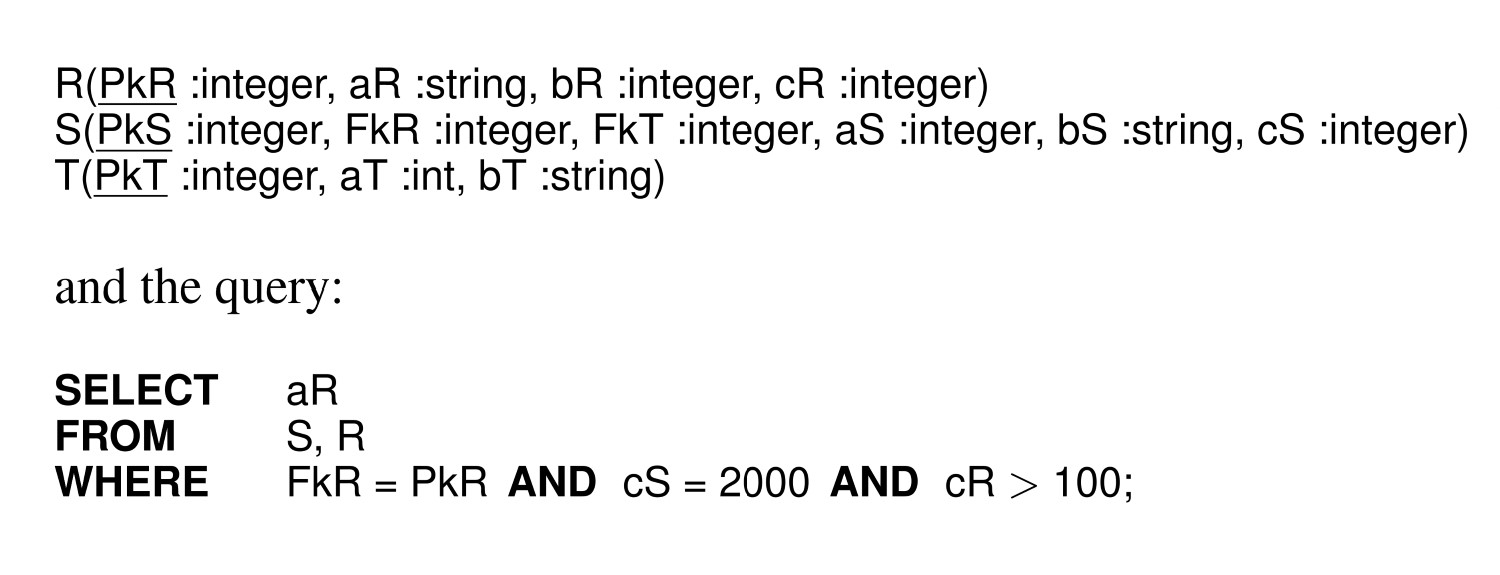
\includegraphics[scale = 0.7]{img/queop6.jpg}
		\label{queop4}
\end{figure}

, and let's consider two alternative physical query plans: the first one uses the join operator \textbf{PageNestedLoop}, while the second one uses the available \textbf{indexes}.

\begin{figure}[H]
		\centering
		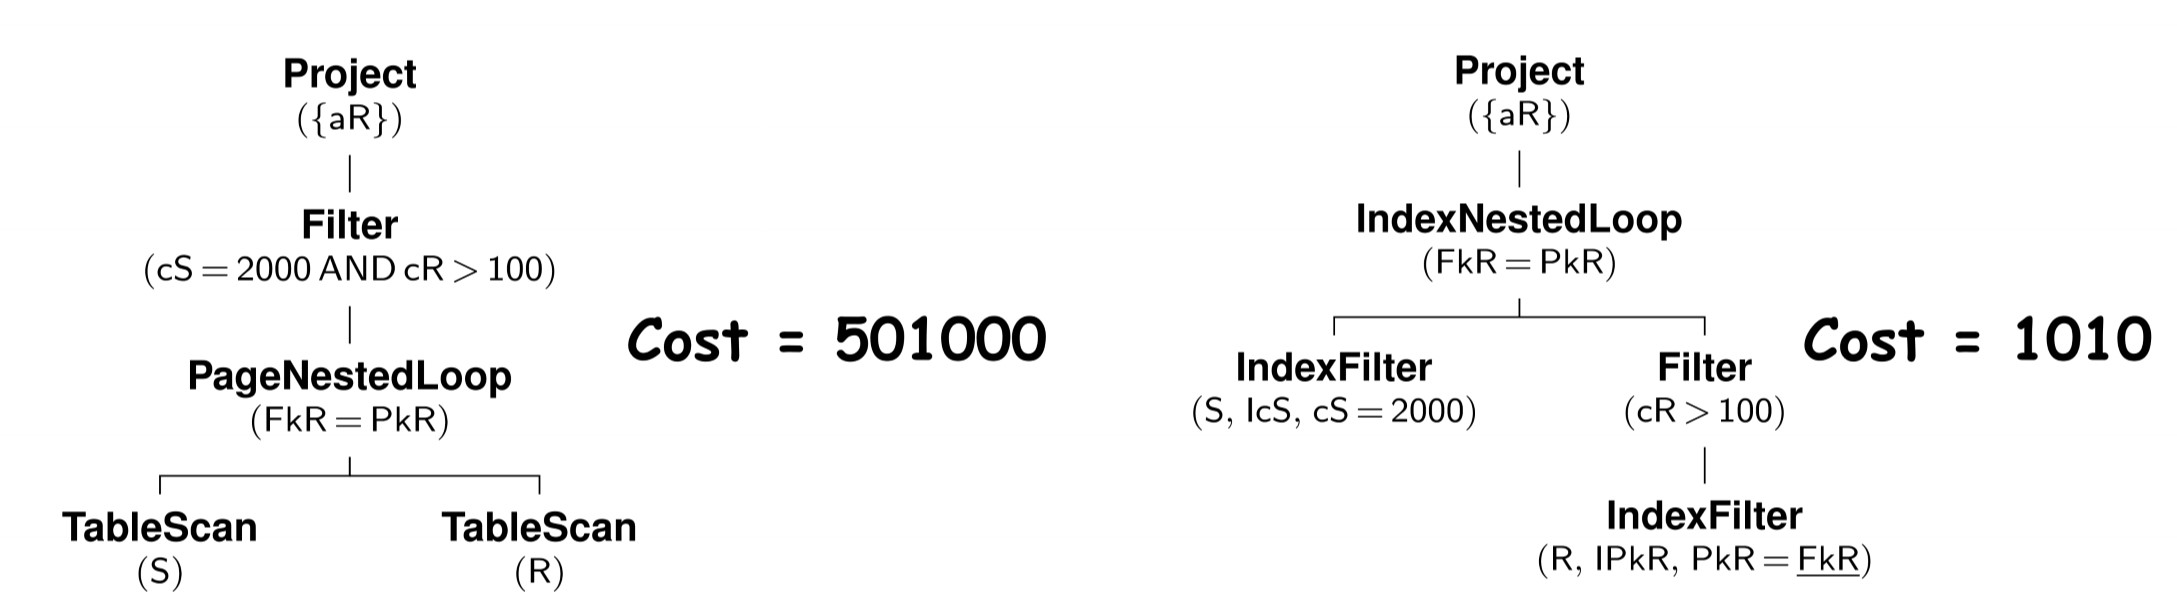
\includegraphics[scale = 0.7]{img/queop7.jpg}
		\label{queop4}
\end{figure}

Clearly, the second physical plan has better performances than the first one.

\subsubsection{Single relation queries}
If the query uses just one relation, the operations involved are the projection and selection.

If there are \textbf{no useful indexes}, the solution is to perform a scan + projection.

Otherwise, if there are useful index we can:

\begin{itemize}
    \item \textbf{use of single-index}: the one of minimal cost is used, and it tests if the record satisfy the conditions and projection is applied. Note that the records of the result are sorted on the index attribute;
    
    \item \textbf{use of multiple-indexes}: the operation is completed by testing whether the retrieved records satisfy the remaining conditions and the projection is applied;

    \item \textbf{use of index-only}: if all the attributes of the condition of the SELECT are included in the prefix of the key of an index, the query can be evaluated using only the index with the query plan of minimum cost.
    
\end{itemize}

\subsubsection{Multiple relation queries}
Queries with two or more relations in the FROM clause require joins (or crossproducts), and finding a good physical query plan for these queries is very important to improve their performances. 

In the following, for simplicity, we will consider an optimization algorithm based on the idea of generating and searching a \textbf{state space} of possible solutions to find the one with minimal cost. The state space is constructed step-by-step starting with an initial state and repeatedly applying a set of operators to expand a state $s$ into other ones, called the \textit{successors} of $s$. Each state $s$ corresponds to a relational algebra subexpression of a given query $Q$ to optimize, and the successors of s are larger subexpressions of Q. The cost of a state $s$ is that of the best physical plan to execute the expression associated to $s$. 

The state space is represented as a tree of nodes, where the root is the empty subexpression, the first level nodes are the query relations or selections and projections on each of them; the following levels are alternative joins of the algebraic expressions of the previous level. The node of the “optimum” state is the expression the contains all the query joins, which is then extended with other operators (e.g. project, sort or group by) to become the final state of the query expression, with the associated minimal cost physical query plan. 

As queries become more complex, the full search algorithm cannot find the overall best physical query plan in a reasonable amount of time because of the \textbf{exponential nature of the problem}. Therefore, several \textbf{heuristics} have been proposed in the DBMS literature that allow the query optimizer to avoid bad query plans and find query plans that, while not necessarily optimal, are usually “good enough”. Some examples are \textit{limitation of the number of successors}, \textit{greedy search} and so on..

\subsubsection{Other queries}

\begin{itemize}

    \item \textbf{DISTINCT queries}: assuming that the operation is performed by sorting, the physical plan for a SELECT ORDER BY is generated, and then extended with the physical operator \textbf{Distinct(O)};
    
    \item \textbf{GROUP BY queries}: the optimizer produces a physical plan for the SELECT only, without considering the GROUP BY clause, which produces the result sorted on the grouping attributes. The physical plan is then extended with a physical operator for the \textbf{GroupBy} and the operator \textbf{Project} over the SELECT attributes. If the SELECT has also a HAVING clause, the physical plan is extended with a selection operator, and the operator \textbf{GroupBy} computes all the aggregate functions used in the HAVING and SELECT clauses;

    \paragraph{Pre-grouping transformation}
    The standard way to evaluate join queries with grouping and aggregations is to perform the join first, but sometimes it is convenient to anticipate grouping operations. However, complex conditions are needed to perform this optimization, which also depends on the type of aggregate functions.

    \item \textbf{Queries with set operations}: we only consider the UNION operator. The optimizer is used to generate the physical plans for the two SELECT of the UNION, with duplicate elimination operators, which then become the operands of the \textbf{Union} operator.

    
\end{itemize}
\section{Transaction and recovery manager}

\begin{figure}[h!]
		\centering
		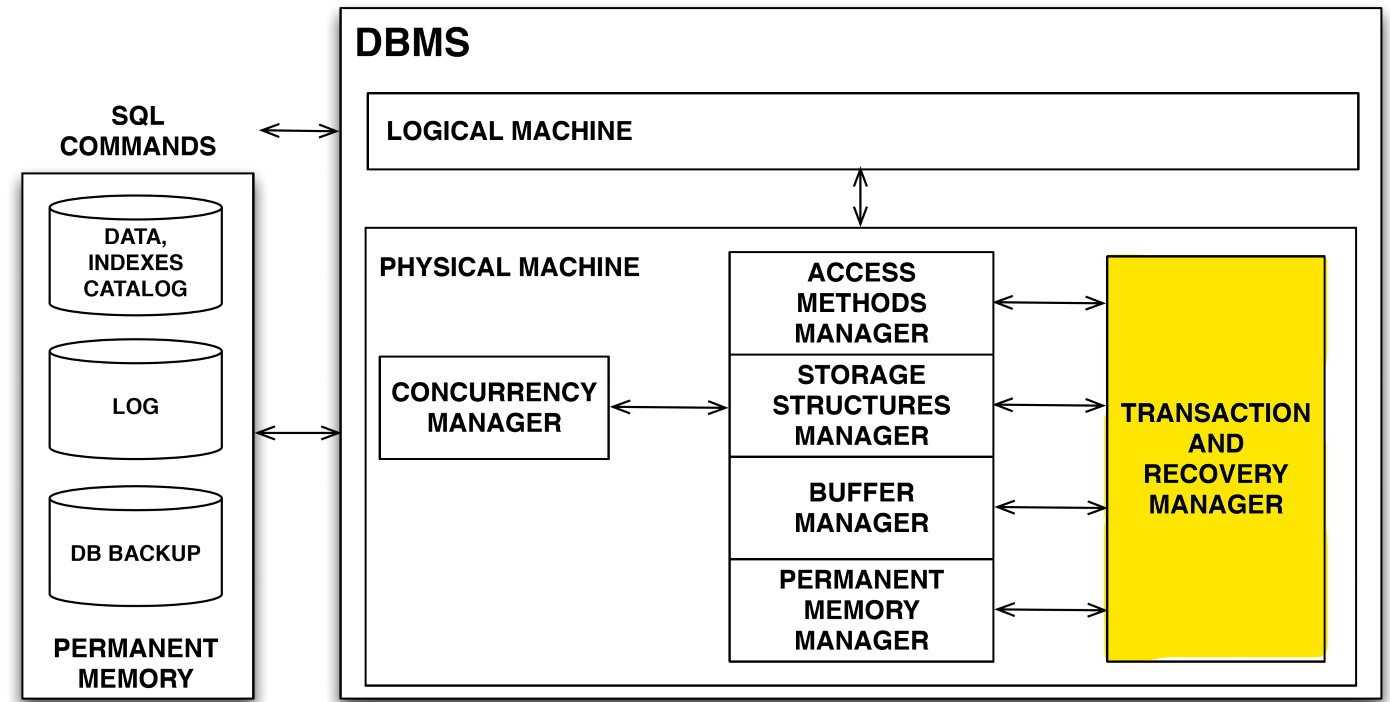
\includegraphics[scale = 0.7]{img/tr1.jpg}
		\label{tr1}
\end{figure}

One of the most important features of a DBMS are the techniques provided for the solution of the \textit{recovery} and \textit{} problems, to allow the users to assume that each of their applications is executed both as if there were no failures, and that there were no interferences with other applications running concurrently. The solutions of these problems are based on the abstraction mechanism called \textit{transaction}. The correct implementation of transactions requires some of the most sophisticated algorithms and data structures of a DBMS. In this chapter we will focus on transactions as a mechanism to protect data from failures, while in the next one we will examine the aspects of transactions concerning the concurrency control to avoid interference.

\subsection{Transactions}
A database is said to be in a \textit{consistent state} if all the integrity constraints are satisfied, and a \textit{transaction} is a mechanism to properly group operations on the database into atomic units of work. A transaction is \textit{correct} if it causes the DB to change from a consistent state to another consistent state, even in a system failure and by handling concurrent transactions.

\subsubsection{Transactions from the programmer's point of view}

\begin{tcolorbox}
A \textbf{transaction} is a sequence of operations on the DB with the following ACID properties:

\begin{itemize}
    \item \textbf{atomicity}: only transactions terminated normally (\textit{committed transactions}) change the database, otherwise the database remains unchanged;

    \item \textbf{isolation}: when a transaction is executed concurrently with others, the final effect must be the same as if it was executed alone;
    
    \item \textbf{durability} the effects of committed transactions on the DB survive system and media failures.
    
\end{itemize}

\end{tcolorbox}

\textbf{NOTE}: 

\begin{itemize}
    \item atomicity, isolation and durability are provided by a DBMS, while consistency cannot be ensured by the system when the integrity constraints are not declared;
    
    \item the isolation property is sometime called the \textit{serializability} property: when a transaction is executed concurrently with others, the final effect must be the same as a serial execution of committed transactions, i.e. the DBMS behaves as if it executes the transactions one at a time;

    \item the \textit{Transaction and Recovery Manager} guarantees the atomicity and durability properties, while the isolation property is guaranteed by the \textit{Concurrency Manager}
    
\end{itemize}


\subsubsection{Transactions from the DBMS's point of view}

\begin{tcolorbox}
A \textbf{transaction} for the DBMS is a sequence of read and write operations which start and end with the following transaction operations: 

\begin{itemize}
    \item \textit{beginTransaction}: beginning of the transaction;
    \item \textit{commit}: successful termination of the transaction and the system has to make its updates durable;
    \item \textit{abort}: abnormal termination, the system has to undo its updates.
\end{itemize}

\end{tcolorbox}

\textbf{NOTE}: the execution of the \textit{} operation does not guarantee the successful termination of the transaction, because it is possible that the transaction updates cannot be written to the permanent memory, and therefore it will be aborted.

Picture \ref{tr2} shows the different states of a transaction execution.

\begin{figure}[h!]
		\centering
		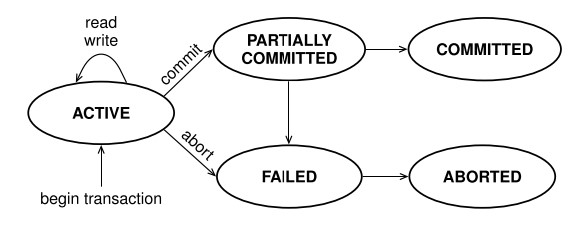
\includegraphics[scale = 1.3]{img/tr2.jpg}
		\label{tr2}
\end{figure}

\begin{itemize}

    \item a transaction enters into the \textit{active} state immediately after it starts execution, where it stays while it is executing;
    
    \item a transaction moves to the \textit{partially committed} state when it ends;
    
    \item a transaction moves to the \textit{committed} state if it has been processed successfully and all its updates on the database have been made durable. In this state we have the warranty that durability is guaranteed;    
    
    \item a transaction moves to the \textit{failed} state if it cannot be committed or it has been interrupted after a transaction failure while in the active state;
    
    \item a transaction moves to the \textit{aborted} state if it has been interrupted and all its updates on the database have been undone. In this state we have the warranty that atomicity is granted.
    
\end{itemize}

Note that the read/write and commit operations are executed by the system when required by the transaction, while the abort operation is executed by the system either when required by the transaction or when a system failure occurs, independently from the transaction requests.

\subsection{Types of failures}
We assume that the occurrence of a failure is always detected, and this causes:

\begin{itemize}
    \item the immediate interruption of a transaction or of the whole system;
    \item the execution of specific \textit{recovery procedures} to ensure that the DB only contains the updates produced by committed operations.
\end{itemize}

The following failures may occur:

\begin{itemize}

    \item \textbf{transaction failures}: is an interruption of a transaction which preserves both the buffer and the permanent memory. It may occur either due to system errors or due to error in a constraint;
    
    \item \textbf{system failure}: is a system interruption, where the content of the buffer is lost, but content of the permanent memory remains intact. In this case the DBMS is restarted;
    
    \item \textbf{media failure}: is an interruption of the DBMS in which the content of the permanent memory is corrupted or lost. In this case the recovery manager uses a backup to restore the DB.
    
\end{itemize}

\subsection{Database system model}
Looking at \ref{tr1} we notice that the permanent memory consists of three main components: the DB, the Log and the DB backup, which are used by the recovery procedure in the case of failures. Note that these three components are stored in distinct physical devices.

The \textit{Transaction and Recovery Manager} performs the following tasks:

\begin{itemize}

    \item execution of read, write, commit and abort operation on behalf of transactions and by cooperating with the \textit{Permanent Memory Manager}, the \textit{Buffer Manager} etc..;

    \item management of the log;

    \item execution of a \textit{restart} command after a system failure, in order to guarantee that the DB only contains the updates of the committed transactions;

    \item execution of techniques to prevent data loss.
    
\end{itemize}

In the next sections the data structures and algorithms used by the recovery manager will be discussed. To simplify the presentation we assume that:

\begin{enumerate}

    \item the database is just a set of pages;
    
    \item each update operation affects a single page, and it is performed by modifying an in-memory copy of the page and then by writing it to disk only when the \textit{Buffer Manager} decide to do it;
    
    \item the operation of transferring a page from the buffer to the permanent memory is an atomic operation;
    
    \item if different transactions are concurrently in execution, they read and write different pages. 
    
\end{enumerate}

\subsection{Data protection}
We saw that there exists different types of failures, but the different techniques that are used in these situations share the common principle of \textbf{redundancy}: to protect the database, the DBMS maintains some redundant information during normal execution of transactions in order to better reconstruct a consistent state, a process called \textbf{recovery}.

\subsubsection{DB backup}
The DBMS provides facilities for periodically making a backup copy of the DB.

\subsubsection{Log}
During the normal use, the history of the operations performed on the database from the last backup is stored in the \textbf{log}. 

\begin{itemize}
    \item for each transaction we write in the log when the transaction starts, commits, aborts and modifies a page;
    \item each log record is identified through the so called \textbf{LSN} (Log Sequence Number), that is assigned in a strictly increasing order. It can be viewed as the serial number of the position of the first character of the record in the file;
\end{itemize}

\begin{figure}[h!]
		\centering
		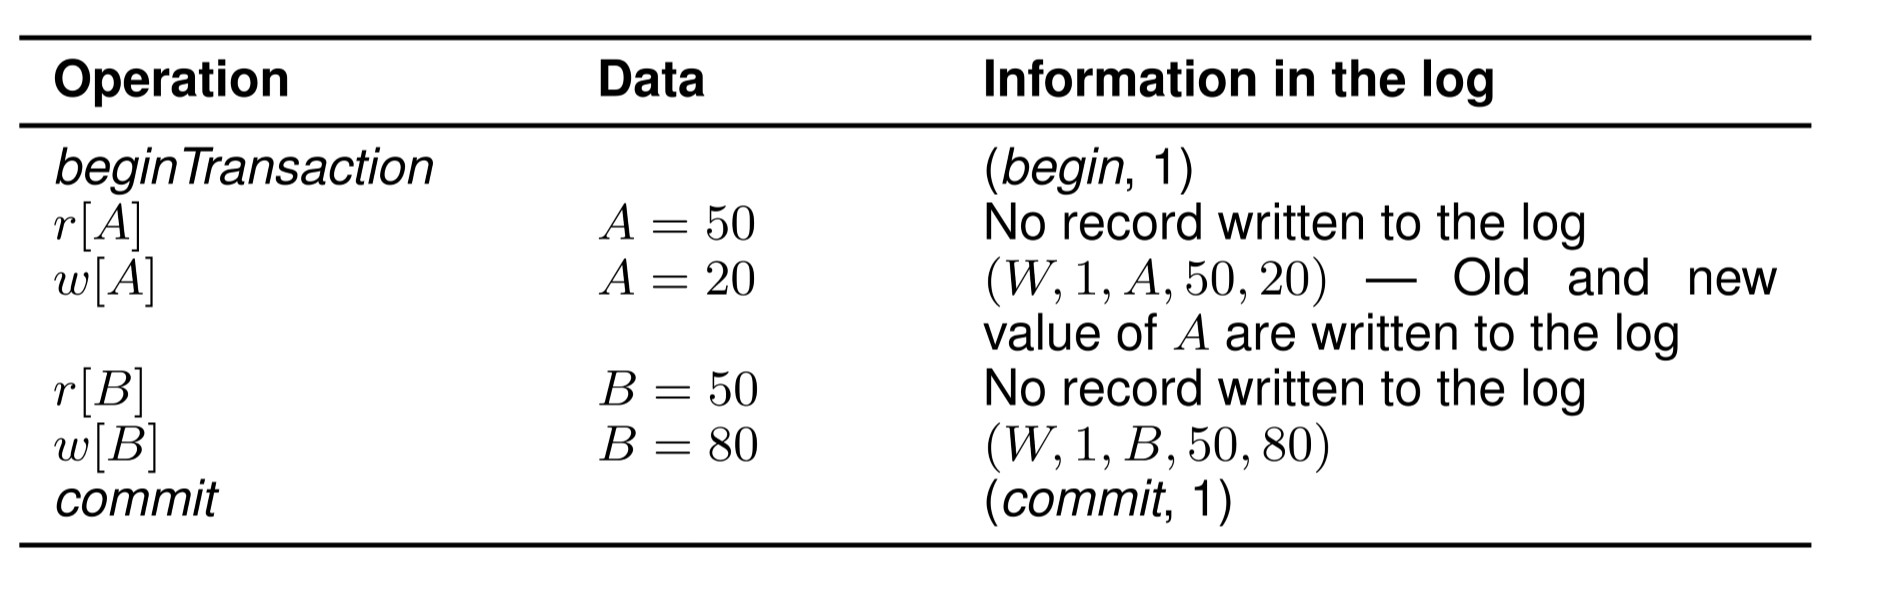
\includegraphics[scale = 0.6]{img/tr5.jpg}
		\label{tr2}
\end{figure}

\textbf{NOTE}:

\begin{itemize}

    \item the read operations do not affect the state of the database, and for this reason no record is written to the log;
    
    \item the exact content of the log depends on the algorithms of the transaction manager;
    
    \item in general a log is stored in a file buffered for efficiency reasons;
    
    \item we assume that the log is not buffered and each record is immediately written to the permanent memory
\end{itemize}

\subsubsection{Undo and Redo algorithms}
Recovery algorithms differ in the information they store in the log, in how they structure this information and, more importantly, in the time when the system transfers the pages updated by a transaction to the permanent memory. We say that a recovery algorithm requires an \textbf{undo} if an update of some uncommitted transaction is stored in the database. Should a transaction or a system failure occur, the recovery algorithm must undo the updates by copying the before-image of the page from the log to the database. 

\begin{figure}[h!]
		\centering
		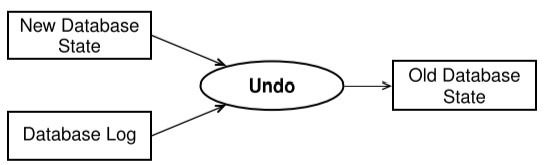
\includegraphics[scale = 1.3]{img/tr3.jpg}
		\label{tr2}
\end{figure}


We say that a recovery algorithm requires \textbf{redo} if a transaction is committed before all of its updates are stored in the database. Should a system failure occur after the transaction commits but before the updates are stored in the database, the recovery algorithm must redo the updates by copying the after-image of the page from the log to the database. 

\begin{figure}[H]
		\centering
		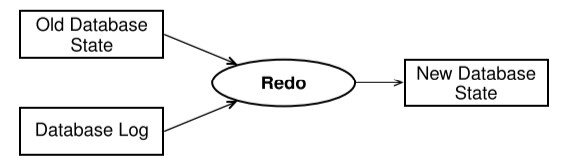
\includegraphics[scale = 1.3]{img/tr4.jpg}
		\label{tr2}
\end{figure}

A failure can happen also during the execution of a recovery procedure, and this requires the restart of the procedure. This means that for such procedures the \textit{idempotency} property must hold. That is, even if the operation is executed multiple times the effect is the same as if it is executed once. For the assumption that the entire page
is replaced, this property is automatically fulfilled.

\subsubsection{Checkpoint}
To reduce the work performed by a recovery procedure in the case of system failure, another information is written to the log, the so called \textbf{checkpoint} (CKP) event. There exists three methods of performing and recording checkpoints:

\begin{itemize}
    \item \textbf{commit-consistent checkpoint}:
    
    \begin{enumerate}
        \item the activation of new transactions is suspended 
        \item the systems waits for the completion of all active transactions
        \item all modified pages present in the buffer (dirty pages) are written to the permanent memory and the relevant records are written to the log. Here the permanent memory is forced so that all the transactions terminated before the checkpoint have their updates
        \item the CKP record is written to the log 
        \item a pointer to the CKP record is stored in a special file, called restart file.
        \item the system allows the activation of new transactions
        
    \end{enumerate}

    This strategy is simple but not efficient, because from (2) we derive that if we have long-time running transactions, we must wait a long time before the flushing of the dirty pages. This problem also affects the work that must be done in the case of restart. For this reason, we should perform this strategy when no transactions are running, but this condition is very demanding;

    \item \textbf{buffer-consistent checkpoint - Version 1}: in this case there's no waiting for active transactions termination, but the problem of the buffer flush operation (costly operation) is still present;

    \item \textbf{Fuzzy checkpoint (ARIES method)}

\end{itemize}

\subsection{Recovery algorithms}
The Recovery managers for the transactions management differ in the way they combine the undo and redo algorithms in order to recover the last consistent state of a DB. There are four possibilities: Undo-Redo, Undo-NoRedo, NoUndo-Redo, NoUndo-NoRedo. In the following sections we assume that a write in the log is forced to disk.

\subsubsection{Use of the Undo algorithm}
The use of the undo algorithm depends on the policy used to write pages updated by an active transactions to the DB:

\begin{itemize}

    \item \textit{deferred update} requires that updated pages cannot be written to the DB before the transaction has committed, and it is implemented by "pinning" the pages in the buffer until the end of the transaction. This policy is costly at the time of the commit, but it is more efficient from the point of view of the resource usage. An algorithm that adopts this policy is a \textit{NoUndo} type: when a system failure occurs, no undo is necessary since the DB has not been changed.

    \item \textit{immediate update} allows that updated pages can be written to the DB before the transaction has committed, and it is implemented by setting the page as "dirty" and by removing its pin. An algorithm that adopts this policy is a \textit{Undo} type: if a system failure occurs, the updates of the DB must be undone.
    
\end{itemize}

To \textbf{undo} the updates of a transaction, the following rule must be observed:

\begin{tcolorbox}[title = Undo rule (Write ahead log)]
    If a database page is updated before the transaction has committed, its before-image must have been previously written to the log file in the permanent memory.
\end{tcolorbox}

This rule allows an undo of a transaction in the case of abort by using the before-images from the log.

\subsubsection{Use of the Redo algorithm}

The use of the redo algorithm depends on the policy used to commit a transaction:

\begin{itemize}

    \item \textit{deferred commit} requires that all updated pages are written to the DB before the commit record has been written to the log. A transaction that implements this policy is a \textit{NoRedo} type: when a system failure occurs, no redo of the updates is necessary. A downside of this policy is that the buffer manager is forced to flush to the permanent memory all the updated pages before the commit operation;

    \item \textit{immediate commit} allows the commit record to be written to the log before all updated pages have been written to the DB. An algorithm that adopts this policy is a \textit{Redo} type, since it is necessary to redo all the updates in the case of a system failure. On the other hand, the buffer manager is free to flush the unpinned pages to the permanent memory when it considers appropriate.

\end{itemize}

To \textbf{redo} the updates of a transaction, the following rule must be observed:

\begin{tcolorbox}[title = Redo rule (commit rule)]
    Before a transaction can commit, the after-images produced by the transaction must have been written to the log file in the permanent memory.
\end{tcolorbox}

\subsubsection{No use of Undo and Redo algorithms}

\begin{itemize}
    \item NoUndo algorithm requires that all the updates of a transaction must be in the database after the transaction has committed;
    \item NoRedo algorithm requires that all the updates of a transaction must be in the database before the transaction has committed
\end{itemize}

Therefore:

\begin{tcolorbox}
     A \textbf{NoUndo-NoRedo} algorithm requires that all the updates of a transaction must be in the database neither before nor after the transaction has committed.
\end{tcolorbox}

This condition is preserved if the commit operation atomically writes all the updates of a transaction to the DB and mark the transactions as committed: this is feasible using the \textbf{shadow pages}. 

The implementation of the shadow pages is based on the \textit{Page table}, a permanent memory index that maps each page identifier to the physical address where the page is stored. Moreover, there is the \textit{descriptor}, which is a record that contains a pointer to the Page table.

\begin{figure}[h!]
		\centering
		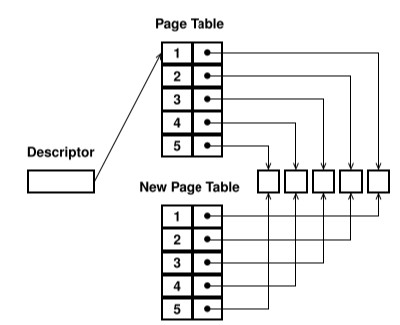
\includegraphics[scale = 1.3]{img/tr6.jpg}
		\label{tr2}
\end{figure}

When a transaction starts, a copy of the Page table is created in the permanent memory (\textit{New page table}), and it is used by the transaction. When a transaction updates for the first time a page: 

\begin{enumerate}
    \item a new database page is created, the \textit{current} page with a certain address $p$, whereas the old page becomes a \textit{shadow page}
    
    \item the New Page Table is updated so that the first element contains the physical address $p$ of the \textit{current page}
\end{enumerate}

\begin{figure}[h!]
		\centering
		\includegraphics[scale = 1.3]{img/tr7.jpg}
		\label{tr2}
\end{figure}


When the transaction reaches the commit point, the system should substitute all the shadow pages with an atomic action, otherwise if a failure happen the database would be left in an incorrect state. This atomic action is implemented by executing the following steps:

\begin{enumerate}
    \item the pages updated in the buffer are written to the permanent memory
    \item the descriptor of the database is updated with an atomic operation
\end{enumerate}

\textbf{NOTE}: 

\begin{itemize}

    \item no need for undo/redo, but this technique is difficult to be applied if the system manages concurrent transactions;
    
    \item if the number of abortion/rollbacks is not high, the undo-redo policy is the preferred one, since it is more efficient.
    
\end{itemize}

\subsection{Recovery from system and media failure}

In the case of \textbf{system failures}, in order to recover the database, the \textit{restart} operator is invoked to perform the following steps (\textit{warm restart}):

\begin{itemize}
    \item bring the database in its committed state with respect to the execution up to the to the system failure;
    \item restart the normal system operations.
\end{itemize}

And is described with two phases: 

\begin{itemize}

    \item in the \textbf{rollback} phase the log is read from the end to the beginning:
    
    \begin{itemize}
    
        \item to undo, if necessary, the updates of the non terminated transactions;
        
        \item to find the set of the identifiers of the transactions which are terminated successfully in order to redo their operations.
        
    \end{itemize}

    \item in the \textbf{rollforward} phase the log is read onward from the first record after the checkpoint to redo all the operations of the terminated transaction
    
\end{itemize}

In this example, both $T_3$ and $T_5$ must be undone, while $T_2$ and $T_4$ must be redone.

\begin{figure}[h!]
		\centering
		\includegraphics[scale = 1.3]{img/tr8.jpg}
		\label{tr2}
\end{figure}

Picture \ref{tr9} and \ref{tr10} show the actions to be performed in the \textit{rollback} and \textit{rollforward} phases of the restart procedure: $L_r$ indicates the set of transactions to be redone, while $L_u$ indicates the set of transactions to be undone.

\begin{figure}[h!]
		\centering
		\includegraphics[scale = 1.3]{img/tr9.jpg}
		\label{tr9}
\end{figure}

\begin{figure}[h!]
		\centering
		\includegraphics[scale = 1.3]{img/tr10.jpg}
		\label{tr10}
\end{figure}

In the case of \textbf{media failure}, a \textit{cold restart} is performed through the following steps:

\begin{itemize}
    \item the most recent database backup is reloaded;
    \item a \textit{rollback} phase is performed on the log;
    \item a \textit{rollforward} phase is performed to update the copy of the database
\end{itemize}


\section{Concurrency management}

\begin{figure}[h!]
		\centering
		\includegraphics[scale = 0.7]{img/conc1.jpg}
		\label{tr10}
\end{figure}

When executing concurrent transactions, some interference may leave the DB in an inconsistent state. The \textit{Concurrency Manager} is the system module that ensures the execution of concurrent transactions without interference during DB access.

\subsection{Introduction}
The problem about concurrent transactions is that their database operations are interleaved, i.e. operations from one program can execute in between operations from another program. This interleaving can cause programs to produce unpredictable results

Assuming that each transaction is \textit{consistent}, a simple way to avoid interference among concurrent transactions is to allow only a \textbf{serial execution}  of them, i.e. all the operations of a transaction are executed before any operation of the other. However, serial executions are impractical from a performance perspective, so we consider a \textbf{serializable execution}. An execution of a set of transactions is \textit{serializable} if its effect is exactly the same as a serial execution of the committed transactions. Serializable executions are \textbf{correct}, because each serializable execution has the same effect of a serial one, and serial executions are correct.

In this sense, the goal of the \textit{Concurrency Manager} is to establish an order among the operations of a set of transactions to make its execution serializable. Its correctness is proved by using the results of the \textbf{serializability theory}, which uses a structure called \textbf{history} (or \textbf{schedule}) to represent the chronological order in which the operations of a set of concurrent transactions are executed, and which goal is to define the properties that an history has to hold to be serializable.

\subsection{Histories}
From the DBMS's point of view, a transaction is seen as a set of read/write/commit and abort operations. For example, this program:

\begin{figure}[h!]
		\centering
		\includegraphics[scale = 0.7]{img/conc2.jpg}
		\label{tr10}
\end{figure}

is seen as $r_1[x]$, $r_1[y]$, $w_1[x]$, $c_1$. 

We make the following assumptions:

\begin{itemize}

    \item a transaction is a set of read/write operations which terminates only with a commit or an abort;
    
    \item we do not consider the operations of insertion or deletion of records;

    \item a transaction reads/writes a specific record at most once.
    
\end{itemize}

We now introduce the concept of history:

\begin{tcolorbox}

 Let $T = \{T_1, T_2, ..., T_n\}$ a set of transaction. A \textbf{history} (or \textbf{schedule}) $H$ on $T$ is an ordered set of operations such that: 

 \begin{enumerate}
     \item the operation of $H$ are those of $T_1, T_2, ..., T_n$
     \item $H$ preserves the ordering between the operations belonging to the same transaction
 \end{enumerate}


\end{tcolorbox}

Intuitively, the history $H$ represents the actual or potential execution order of the operations of the transactions $T_1, T_2, ..., T_n$. An example of history involving three transactions could be the following one:

\begin{figure}[h!]
		\centering
		\includegraphics[scale = 1.5]{img/conc3.jpg}
		\label{tr10}
\end{figure}

\subsubsection{Equivalent histories}

For \textbf{equivalent histories} we could mean that they produce the same effects on the database, namely that the values written to the database by the committed transactions are equal. Since a DBMS knows nothing of the computations made by a transaction in temporary memory, a \textbf{weaker notion} of equivalence which takes into account only the order of operations in conflict made on the database is preferred.

\begin{tcolorbox}
    Two operations of different transactions are in \textbf{conflict} if they are on the same data item and at least one of them is a write operation.
\end{tcolorbox}

This definition allows us to define three types of situations in which the operations are in conflict:

\begin{itemize}

    \item Write-Read Conflict. \\Consider the following piece of a history: $H = ...w1[x],r2[x]...$. The transaction $T_2$ reads $x$ updated by $T_1$ which has not yet committed. This type of read, called \textit{dirty read}, can give rise to executions not serializable;

    \item Read-Write Conflict. \\Consider the following piece of a history: $H = ...r1[x],w2[x],r1[x],...$ Transaction $T_2$ writes a data $x$ previously read by the transaction $T_1$, still active, which then rereads it getting a different value even if in meanwhile $T_1$ has not updated it. This effect obviously can not be achieved by any serial execution of the two transactions;

    \item Write-Write Conflict. \\Consider the following piece of a history: $H = ...w1[x],w2[x]...$ The two transactions, while attempting to modify a data item $x$, both have read the item’s old value before either of them writes the item’s new value. 
    
\end{itemize}

\begin{tcolorbox}
    Two histories $H_1$ and $H_2$ are \textbf{c-equivalent} (conflict-equivalent), i.e. equivalent with respect to operations in conflict, if:
    
    \begin{enumerate}
        \item they are defined on the same set of transactions $T = \{T_1, T_2, ..., T_n\}$ and have the same operations;
        \item they have the same order of operations in conflict of transactions terminated normally
    \end{enumerate}
    
\end{tcolorbox}

Condition (1) requires that $H_1$ and $H_2$ contain the same set of operations to be comparable, while condition (2) requires that $H_1$ and $H_2$ have the same order of the operations in conflict of committed transactions

\subsection{Serializable history}
A history $H$ on the set $T = \{ T_1, T_2, ..., T_n \}$ is \textbf{serial} if it represents a serial execution of $T$ in some order. 

We can now define a stronger condition that is sufficient to ensure that a history is serializable:

\begin{tcolorbox}
    A history $H$ on the transactions $T = \{T_1, T_2, ..., T_n\}$ is \textbf{c-serializable} if it is c-equivalent to a serial history on $T_1, T_2, ..., T_n$.
\end{tcolorbox}

\textbf{NOTE} that each c-serializable history is serializable, but there are serializable histories that are not c-serializable.

\paragraph{Serialization graph}
Another way of examining a history $H$ and decide whether it is c-serializable or not is to analyze a particulare graph derived from $H$, called the \textbf{serialization graph}.

\begin{tcolorbox}
    Let $H$ be a history of committed transactions $T = \{T_1, T_2, ..., T_n\}$. The \textbf{serialization graph} of $H$, denoted $SG(H)$, is a directed graph such as:
    \begin{itemize}
        \item there is a node for every committed transaction in $H$;
        \item there is a directed arc from $T_i \rightarrow T_j$, with $(i \neq j)$ if and only if in $H$ some operation $p_i$ in $T_i$ appears before and conflicts with some operation $p_j$ in $T_j$.
    \end{itemize}

\end{tcolorbox}

We say that two transactions $T_i$ and $T_j$ conflicts if $T_i \rightarrow T_j$ appears in $SG(H)$.

As an example, this is the serialization graph of the given history.

\begin{figure}[h!]
		\centering
		\includegraphics[scale = 1.5]{img/conc4.jpg}
		\label{conc4}
\end{figure}

\begin{figure}[h!]
		\centering
		\includegraphics[scale = 1.5]{img/conc5.jpg}
		\label{conc5}
\end{figure}

\begin{tcolorbox}[title = C-Serializability theorem]
    A history $H$ is c-serializable if and only if its serialization graph $GS(H)$ is acyclic.
\end{tcolorbox}

Since Picture \ref{conc5} represents an acyclic graph, the history in Picture \ref{conc4} is c-serializable!

\subsection{Serializability with locking}

From the analysis of the serialization graph it can be verified a posteriori if a history is c-serializable. Histories and serialization graphs, however, are abstract concepts, and during the execution of a set of transactions, the \textbf{serialization graph is not constructed}. Conversely, the c-serializability theorem is used to prove that the \textbf{scheduling algorithm for the concurrency control} used by a scheduler is correct, i.e. that all histories representing executions that could be produced by it are c-serializable.

\subsubsection{Strict two-phase locking}
A simple scheduling algorithm to obtain serializability is the \textit{Strict 2PL} protocol. The idea behind this approach is simple: each data item used by a transaction has a \textbf{lock} associated with it, which could be:

\begin{itemize}
    \item a \textit{read} or \textit{shared} (S) lock;
    \item a \textit{write} or \textit{exclusive} (X) lock.
\end{itemize}

, and it follows two rules:

\begin{enumerate}

    \item if a transaction $T_i$ wants to read a data item, it first request a shared lock on the data item (first phase):
    
    \begin{itemize}
    
        \item if no other transaction holds the lock, then the data item is locked;
        
        \item if another transaction $T_j$ holds a lock in conflict, then $T_i$ must wait until $T_j$ releases it
        
    \end{itemize}

    
    \item All locks held by a transaction $T_i$ are released together when $T_i$ commits or aborts (second phase). To guarantee the isolation of a transaction, lock releases cannot occur before commit/abortion time.
   
\end{enumerate}

We can describe the \textit{lock-granting policies} of Strict 2PL protocol using a \textbf{compatibility matrix}: 

\begin{itemize}

    \item a row corresponds to a lock that is already held on an element $x$ by another transaction;
    
    \item the columns correspond to the mode of lock on $x$ that is requested
    
\end{itemize}

\begin{figure}[h!]
		\centering
		\includegraphics[scale = 1.5]{img/conc6.jpg}
		\label{conc5}
\end{figure}

\textbf{NOTE}: 
\begin{itemize}

    \item requests to acquire or release locks are automatically inserted into transactions by the \textit{Transaction Manager};
    
    \item lock and unlock requests are handled by the scheduler with the use of the \textit{Lock Table}, in which an entry contains the ID of the data item being blocked, the type of lock granted or requested, a list of transactions holding lock and a queue of lock requests.
    
\end{itemize}

\begin{tcolorbox}[title = C-Serializability of Strict 2PL]
    A \textit{Strict 2PL} protocol ensures c-serializability.
\end{tcolorbox}

However, the set of \textit{Strict 2PL} histories is a subset of the c-serializable histories, i.e. there are c-serializable histories that are not \textit{Strict 2PL}.

\subsubsection{Deadlocks}

Although being simple, \textit{Strict 2PL} needs a strategy to detect \textit{deadlocks}, a situation in which, for example, two transactions lock two different items and none of them can proceed. The deadlock problem can be solved with deadlock prevention techniques or with deadlock detection and recovery technques.

\paragraph{Deadlock detection}

\begin{itemize}

    \item a strategy to detect deadlocks uses a \textbf{wait-for graph}, in which :
    
    \begin{itemize}
    
        \item the nodes are active transactions;
        
        \item an arc from $T_i$ to $T_j$ indicates that $T_i$ is waiting for a resource held by $T_j$.

    \end{itemize}  
    
    Using this representation, a \textbf{cycle} in the graph indicates that a \textbf{deadlock} has occurred, and one of the transactions of the cycle must abort;
    
    \item the standard method to decide which transaction to abort is to choose the \textbf{“youngest”} transaction by some metric (being young, it has probably done less work, so it is less costly to abort);
    
    \item checking for cycles requires a linear complexity algorithm, but the actual cost of the management of the graph in real cases discourage the use. For this reason, instead of wait-for graph we can use the \textbf{timeout strategy}: if a transaction has been waiting too long for a lock, then the scheduler simply presumes that deadlock has occurred and it aborts the transaction.

\end{itemize}

\paragraph{Deadlock prevention}

\begin{itemize}
    \item each transaction $T_i$ receives a timestamp $t_s(T_i)$ when it starts: $T_i$ is older than $T_j$ if $t_s(T_i) < t_s(T_j)$;

    \item each transaction is assigned a priority on the basis of its timestamp: the \textbf{older} a transaction is, the \textbf{higher priority} it has. 
    
    \item when a transaction $T_i$ requests a lock on a data item that conflicts with the lock currently held by another active transaction $T_j$, two algorithms are possible:

    \begin{enumerate}
    
        \item wait-die (or non-preemptive technique): an older transaction waits only for a younger one, otherwise the younger dies.
        
        \item wound-wait (or preemptive technique): an older transaction wounds a younger one to take its lock, otherwise the younger waits for the older one.
        
    \end{enumerate}
    
    
    In both cases when an aborted transaction $T_i$ is restarted, it has the same priority it had originally: this property ensures that sooner or later every transaction will become the oldest, so it ensures that no \textit{starvation} will occur.

    These two algorithms have the property of \textbf{not creating deadlocks}, but their behaviour is very different:

    \begin{itemize}

        \item with the wait-die method, a transaction $T$ can wait for data locked by a younger transaction or it restarts due to an older one $T_0$. Most likely is the second case and then the method favors the restarting rather than waiting;
    
        \item with the wound-wait method, a transaction $T$ can wait for data locked by an older transaction or restarts a younger one $T_y$. Most likely is the first case followed by the waiting rather than restarting.
        
    \end{itemize}

    \item deadlock prevention methods are easier to implement than deadlock detection solutions, but on the other hand they lead to the abortion of transactions which could run without restarts.
    
\end{itemize}

\subsection{Serializability without locking}
While methods of concurrency control that use locks are called \textit{pessimistic}, in the sense that they're based on the idea that a bad things is likely to happen, other methods, called \textit{optimistic}, do not lock data because are based on the idea that bad things are not likely to happen. However, in this approach, when a transaction requests to commit, the system controls that no bad things has happened.

\paragraph{Snapshot isolation}

\begin{itemize}

    \item a transaction can perform any database operation without requesting permission, and taking advantage of \textit{multiversions} of each data item;
    
    \item the transactions must request permission to commit;

    \item each transaction $T_i$ reads the data of the DB version (\textit{snapshot}) produced by all the transactions committed before $T_i$ starts, but no effects are seen of other concurrent transactions. 

    \item this approach grants that no concurrent writes are performed ("First-Committer-Wins" rule).
    
\end{itemize}

\subsection{Multiple granularity locking}
The concurrency control techniques seen so far, based on the idea of a single record lock, is not sufficiently general to treat transactions that operate on collections of records. For example, in some cases it could be convenient to lock an entire table, rather that a single record. 

For this reason, other techniques are base on the idea that the data to lock can have different \textbf{granularities}, and among them is defined an inclusion relationship : $\text{DB} \rightarrow \text{Files} \rightarrow \text{Pages} \rightarrow \text{Records} \rightarrow \text{Fields}$.

The inclusion relation between data can be thought of as a \textbf{tree} of objects where each node contains all its children. If a transaction gets an \textit{explicit} $S$ or $X$ lock on a node, then it has an \textit{implicit} lock in the same lock mode on all the descendants of that node.

In order to manage locks on data of different granularities, \textit{intention locks} are introduced: 

\begin{tcolorbox}[title = Multiple-granularity and intention locks]
    Multiple-granularity locking requires that before a node in explicitly locked, a transaction must first have a proper intention lock on all the ancestors of that node in the granularity hierarchy. 
\end{tcolorbox}

The intention locks are the following:

\begin{itemize}

    \item $IS$, or \textit{intention shared lock}, allows requestor to explicitly lock descendant nodes in $S$ or $IS$ mode;

    \item $IX$ or \textit{intention exclusive lock}, allows requestor to explicitly lock descendants in $S$, $IS$, $X$, $IX$ or $SIX$ mode;
    
    \item $SIX$ or \textit{shared intentional exclusive lock}, implicitly locks all descendants of node in $S$ mode and allows requestor to explicitly lock descendant nodes in $X$, $SIX$, or $IX$ mode.
    
\end{itemize}

Note that the $SIX$ lock is introduced in order to combine $S$ and $IX$ to simplify the lock manager, since they frequently appera together.

The compatibility matrix is:

\begin{figure}[h!]
		\centering
		\includegraphics[scale = 1.5]{img/conc7.jpg}
		\label{conc5}
\end{figure}

To deal with multiple granularity locks, it is necessary extend the \textit{Strict 2PL protocol} with new rules, obtaining the protocol called \textbf{Multi-granularity Strict 2PL}:

\begin{enumerate}

    \item a node can be locked by a transaction $Ti$ in $S$ or $IS$ mode only if the parent is locked by $Ti$ in $IS$ or $IX$ mode.
    
    \item a node can be locked by a transaction $Ti$ in $X$, $IX$ or $SIX$ mode only if the parent is locked by $Ti$ in $SIX$ or $IX$ mode.

\end{enumerate}

\subsection{Locking for dynamic databases}

So far we have considered only transactions that read or update existing records in the database. In reality, transactions can also \textbf{insert} or \textbf{delete} records into tables with \textbf{indexes}. These possibilities raise new problems to be solved to ensure serializability during the concurrent execution of a set of transactions, while continuing to adopt the Strict 2PL protocol.

\paragraph{Insertion and Deletion}
The inserted or deleted records are called \textit{phantoms} because they are records that appear or disappear from sets, i.e. they are invisible only during a part of a transaction execution. 

An acceptable practical solution to this problem is \textbf{index locking}. When a set of records that match some predicate is locked, the database system also checks to see if there is an index whose key matches the predicate. If such an index exists, the structure of the index should allow us to easily lock all the pages in which new tuples that match the predicate appear or will appear in the future. The practical issue of how to locate the relevant pages in the index that need to be locked and what locks need to be acquired is discussed in the following section.

\paragraph{Concurrency Control in B+–trees}

The concurrent use of a B+–tree index by several transactions may be treated in a simple way with \textit{Strict 2PL protocol}, by considering each node as a granule to lock appropriately. This solution, however, would lead to a low level of concurrency due to locks on the first tree levels. 

A better solution is obtained by exploiting the fact that the indexes are used in a particular way during the operation. In the case of a search, the nodes visited to reach the leaves, where the data is located, are locked in reading during the visit and unlocked as soon as the search proceeds from one node to the child. In the case of an insertion, during the visit of the tree when switching from one node $A$ to a child $B$ not full, the locks on $A$ can be released because a possible propagation of the effect of the insert into a leaf stops at node $B$, called a (safe node). A node is safe for a delete operation if it is at least half full. The general case with node splits, merging and balancing is more complex and several tree locking techniques have been proposed. 



\end{document}